\documentclass[a4paper,12pt]{article}


\setlength{\textwidth}{15.0cm}
\setlength{\textheight}{24.0cm}
\setlength{\topmargin}{0cm}
\setlength{\headsep}{0cm}
\setlength{\headheight}{0cm}
\pagestyle{plain}

\usepackage[dvips]{epsfig}
\usepackage{tikz}

\usepackage[
backend=biber,
style=alphabetic,
]{biblatex}

\usepackage{amsmath,amssymb,amsthm}
\newtheoremstyle{break}{4pt}{4pt}{}{}{\bfseries}{\vspace{2 pt}}{\newline}{}
\theoremstyle{break}
\newtheorem{theorem}{Theorem}[subsection]
\newtheorem{example}[theorem]{Example}
\newtheorem{definition}[theorem]{Definition}
\newtheorem{notation}[theorem]{Notation}
\newtheorem{lemma}[theorem]{Lemma}
\newtheorem{corollary}[theorem]{Corollary}
\newtheorem{technique}[theorem]{Technique}
\newtheorem{pythonn}[theorem]{Python Code}
\newtheorem{related}[theorem]{Related Work}

\usepackage{comment}
\usepackage{listings}
% Define custom colors for Python syntax highlighting
\definecolor{codebackground}{RGB}{242, 242, 242}
\definecolor{codecomment}{RGB}{106, 153, 85}
\definecolor{codekeyword}{RGB}{0, 0, 255}
\definecolor{codestring}{RGB}{170, 55, 241}

% Define custom Python style for syntax highlighting
\lstdefinestyle{custompython}{
    language=Python,
    backgroundcolor=\color{codebackground},
    basicstyle=\ttfamily\footnotesize,
    commentstyle=\color{codecomment}\itshape,
    keywordstyle=\color{codekeyword}\bfseries,
    stringstyle=\color{codestring},
    showstringspaces=false,
    breaklines=true,
    breakatwhitespace=true,
    tabsize=4,
    frame=tb,
    framesep=4pt,
    framerule=0.5pt,
    numbers=left,
    numbersep=10pt,
    numberstyle=\footnotesize\color{gray},
    xleftmargin=15pt,
    xrightmargin=5pt,
    aboveskip=5pt,
    belowskip=5pt,
    captionpos=b
}

\newcommand{\pythoncode}[1]{
    \hspace*{0cm}
    \vspace{-0.3cm}
    \lstinputlisting[style=custompython]{#1}}

% Define custom colors for Julia syntax highlighting
\definecolor{juliabackground}{RGB}{240, 230, 255} % Light purple background
\definecolor{juliacomment}{RGB}{128, 0, 128}     % Purple comments
\definecolor{juliakeyword}{RGB}{75, 0, 130}      % Indigo keywords
\definecolor{juliastring}{RGB}{147, 112, 219}    % Medium purple strings

% Define custom Julia style for syntax highlighting
\lstdefinelanguage{Julia}%
{
    morekeywords={
            abstract, break, case, catch, const, continue, do, else, elseif, end,
            export, false, for, function, global, if, immutable, import, importall,
            in, macro, module, otherwise, quote, return, switch, true, try, type,
            typealias, using, while
        },
    sensitive=true,
    alsoother={$},
    morecomment=[l]\#,
    morecomment=[n]{\#=}{=\#},
    morestring=[s]{"}{"},
    morestring=[s]{'}{'},
}[keywords,comments,strings]

\lstdefinestyle{customjulia}{
    language=Julia,
    backgroundcolor=\color{juliabackground},
    basicstyle=\ttfamily\footnotesize,
    commentstyle=\color{juliacomment}\itshape,
    keywordstyle=\color{juliakeyword}\bfseries,
    stringstyle=\color{juliastring},
    showstringspaces=false,
    breaklines=true,
    breakatwhitespace=true,
    tabsize=4,
    frame=tb,
    framesep=4pt,
    framerule=0.5pt,
    numbers=left,
    numbersep=10pt,
    numberstyle=\footnotesize\color{gray},
    xleftmargin=15pt,
    xrightmargin=5pt,
    aboveskip=5pt,
    belowskip=5pt,
    captionpos=b,
    columns=flexible,
    keepspaces=true
}

\newcommand{\juliacode}[1]{
    \hspace*{0cm}
    \vspace{-0.3cm}
    \lstinputlisting[style=customjulia]{#1}
}

\addbibresource{bibliography.bib} 
\setlength{\parindent}{0pt}

\begin{document}

\begin{comment}
\title{Recursive Monte Carlo}
\author{Isidoor Pinillo Esquivel}
\maketitle
\end{comment}

\begin{titlepage}
    \begin{center}
        \resizebox{3cm}{!}{
\includegraphics{./vert2_kl_01.eps}}
        \ \
        \ \\
        \ \\
        \ \\
        \ \\
        \ \\
        \ \\
        \ \\
        \ \\
        \ \\
        \ \\
        \ \\
        \Large{M{\sc asterproef scriptie}}
        \ \\
        \ \\
        \ \\
        \huge{\bf{\em Recursive Monte Carlo for linear ODEs}}
        \ \\
        \ \\
        \ \\
        % \ \\
        \ \\
        \ \\
        \normalsize
        Auteur: {\em Isidoor Pinillo Esquivel}\\
        \ \\
        \ \\
        Promotor: {\em Wim Vanroose}\\
        \ \\
        \ \\
        \ \\
        \ \\
        \ \\
        \ \\
        \ \\
        A{\sc cademiejaar 2022-2023}

    \end{center}
\end{titlepage}




\newpage
\tableofcontents
\newpage

\begin{abstract}
    We will write this at the end. Also need a dutch abstract
\end{abstract}

\section{Introduction}

\subsection{Introductory Example}
In this subsection we introduce recursive  Monte Carlo with our main example
for IVPs:

\begin{equation} \label{ydy}
    y'=y, y(0)=1.
\end{equation}

Integrating both sides of (\ref{ydy}) obtains:

\begin{equation} \label{Integral ydy}
    y(t) = 1 + \int_{0}^{t} y(s) ds.
\end{equation}

Equation (\ref{Integral ydy}) is a recursive integral equation or to be more specific
a linear Volterra integral equation of the second type. By estimating the recursive integral
of equation (\ref{Integral ydy}) with Monte Carlo one derives following estimator:

\begin{equation}
    Y(t) = 1 + t y(Ut).
\end{equation}

With $U \sim \text{Uniform}(0,1)$. If $y$ is well behaved then $E[Y(t)]=y(t)$ but we can't
calculate $Y(t)$ without accesses to $y(s),s<t$. Notice that we can replace $y$ by a
unbiased estimator of it without changing $E[Y(t)]=y(t)$ by the law of total expectance
($E[X] = E[E[X|Z]]$). By replacing $y$ by $Y$ itself we obtain a recursive expression for $Y$:

\begin{equation}\label{recursive RV}
    Y(t) = 1 + tY(Ut).
\end{equation}

Equation (\ref{recursive RV}) is a recursive random variable equation (RRVE). If you would implement equation
(\ref{recursive RV}) with recursion it will run indefinitely. A biased way of around this is by approximating
$Y(t) \approx 1$ near $t = 0$. Later we discuss Russian roulette (\ref{Russian roulette}) which
can be used as an unbiased stopping mechanism.

\vspace*{0.2cm}

\begin{pythonn}[implementation of (\ref{recursive RV})] \label{python eps ydy}
    \pythoncode{python code/eps_ydy.py}
    To gain insight into realizations of RRVEs, it can be helpful to plot
    all recursive calls $(t,Y(t))$, as shown in Figure \ref{fig:intro example}
    for this implementation.

    \begin{figure}[h!]
        \centering
        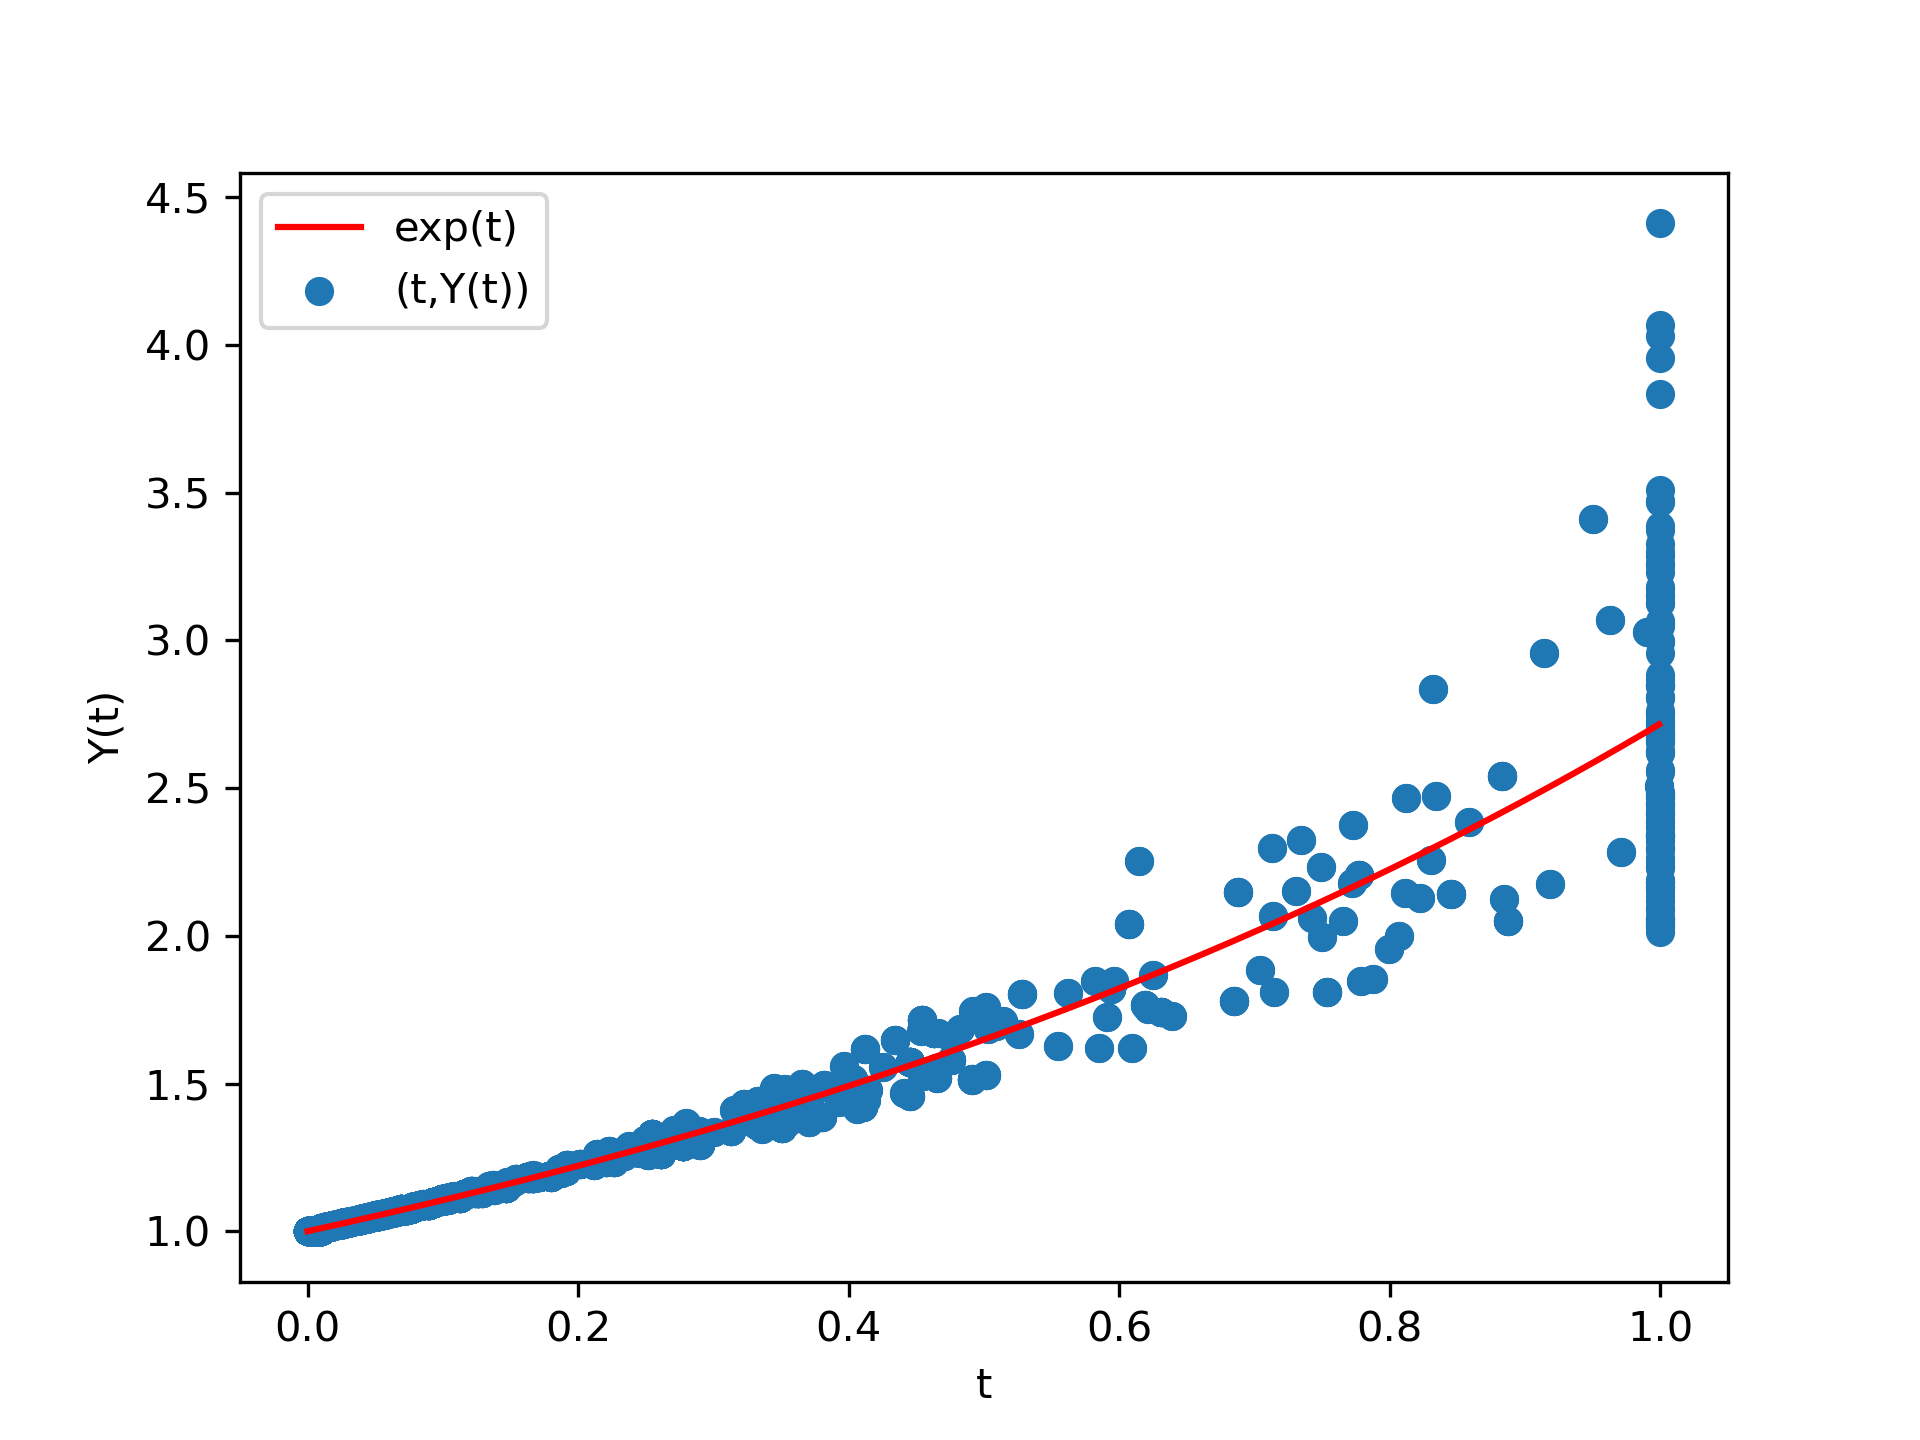
\includegraphics[width=0.8\textwidth]{plots/intro example.png}
        \caption{Recursive calls of (\ref{python eps ydy})}
        \label{fig:intro example}
    \end{figure}
\end{pythonn}

An issue with (\ref{python eps ydy}) is that the variance increases rapidly when $t$ increases. Later
this is issue gets resolved in the section on ODEs. Note that (\ref{python eps ydy}) keeps desirable properties
from unbiased Monte Carlo methods such as being embarrassingly parallel and
having simple error estimates.

\subsection{Related Work}
work on
\begin{itemize}
    \item alternative methods for recursive integrals
    \item MC work on ODEs
    \item MC work on PDEs
    \item WoS
\end{itemize}
This is just to give a general overview we probably reference specific ideas when we first introduce them.

\subsection{Contributions}
We write this at the end. Probably a lot of conjectures.


\section{Background}

\subsection{Notation}
Notations used in this thesis include:

\begin{itemize}
    \item $U \sim \text{Uniform}(0,1)$.
    \item $B(p) \sim \text{Bernoulli}(p)$.
    \item RV = random variable.
    \item RVs will be denoted with capital letters, e.g., $X,Y$ or $Z$.
    \item RRVE (recursive RV equation): An equation that defines a
          family of random variables in terms of its self.
    \item MC = Monte Carlo.
    \item RMC = Recursive MC.
    \item RRMC = Recursion in Recursion MC.
\end{itemize}


\subsection{Modifying Monte Carlo}
In this subsection, we discuss techniques for modifying RRVEs
in a way that preserves the expected value of the solution while
acquiring more desirable properties. \\

Russian roulette is a MC technique commonly used in rendering.
The main idea behind Russian roulette is to replace a random variable
with a less computationally expensive approximation sometimes.

\begin{definition}[Russian roulette] \label{Russian roulette}
    Define Russian roulette on $X$ with free parameters
    $Y_{1},Y_{2}: E[Y_{1}] = E[Y_{2}]$, $p \in [0,1]$ and $U$
    independent of $Y_{1},Y_{2},X$ the following way:
    \begin{equation}
        X \rightarrow \begin{cases}
            \frac{1}{p}(X- (1-p)Y_{1}) & \text{ if } U<p \\
            Y_{2}                      & \text{ else }
        \end{cases}.
    \end{equation}
\end{definition}

\begin{example}[Russian roulette]
    Say that we are interested in estimating $E[Z]$ with $Z$
    defined in the following way:
    \begin{equation}
        Z = U + \frac{f(U)}{1000}.
    \end{equation}
    where $f:\mathbb{R} \rightarrow [0,1]$ expensive to compute.
    Estimating $E[Z]$ directly would require calling $f$ each
    simulation. We can modify $Z$ to
    \begin{equation}
        \tilde{Z} = U + B\left(\frac{1}{100}\right)\frac{f(U)}{10}.
    \end{equation}
    Now $\tilde{Z}$
    just requires calling $f$ on average once every $100$ simulations with the variance
    only increasing slightly compared to $Z$. \\

    In this example it is also possible to estimate the expectance of the $2$
    terms of $Z$ separately.
\end{example}

\begin{example}[Russian roulette on (\ref{recursive RV})]
    Russian roulette can fix the indefinite recursion issue of
    equation (\ref{recursive RV}) by approximating $Y$ near $t = 0$ with $1$
    sometimes. Concretely
    we replace the $t$ in front of the recursive term with $B(t)$
    when $t<1$.
    \begin{equation}
        Y(t) =
        \begin{cases}
            1 + B(t)Y(Ut) & \text{ if } t<1 \\
            1 + tY(Ut)    & \text{ else}
        \end{cases}.
    \end{equation}
\end{example}

\vspace{0.2cm}

\begin{pythonn}[Russian roulette on (\ref{recursive RV})] \label{RRpython}
    \pythoncode{python code/RR_ydy.py}
    Interestingly, $Y(t)$ is constrained to take on only integer values.
    This is visually evident on Figure \ref{fig:russian roulette}.
    \begin{figure}[h!]
        \centering
        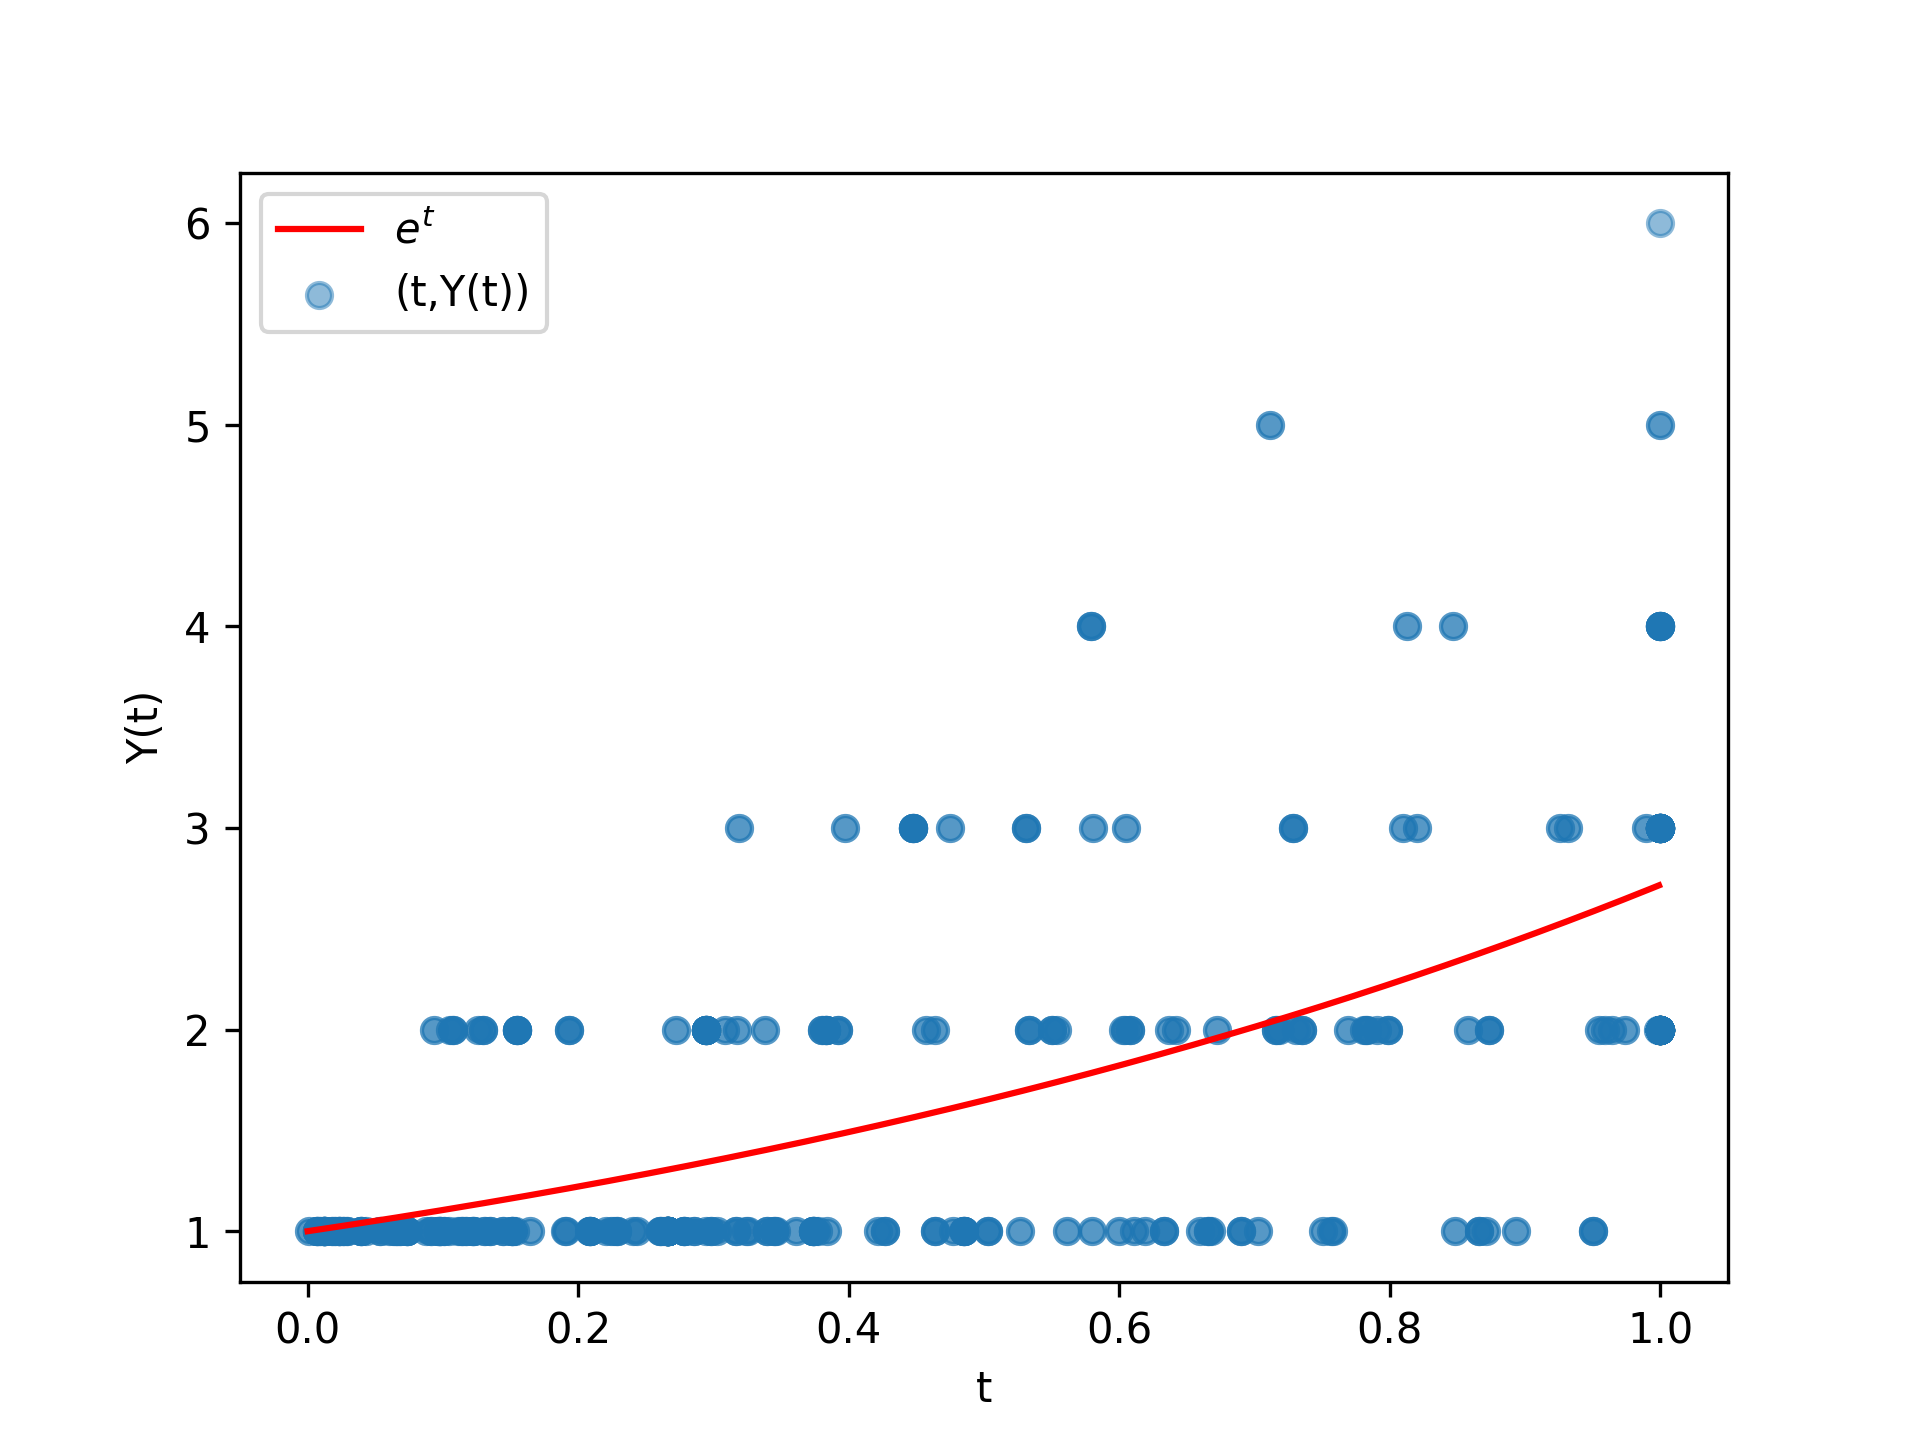
\includegraphics[width=0.8\textwidth]{plots/russian roulette example.png}
        \caption{Recursive calls $(t,Y(t))$ of (\ref{RRpython}) }
        \label{fig:russian roulette}
    \end{figure}

\end{pythonn}

Splitting is a technique that has almost the reverse effect of Russian roulette.
Instead of reducing the number of simulations of a RV as Russian roulette does,
we increase it by using more samples (i.e., splitting the samples) which
reduces the variance.

\begin{definition}[splitting] \label{def:splitting}
    Splitting $X$ means using multiple $X_{j} \sim X$ not independent per se to
    lower variance by averaging them:
    \begin{equation}
        \bar{X}= \frac{1}{N} \sum_{j=1}^{N} X_{j}.
    \end{equation}
\end{definition}

Splitting the recursive term in a RRVE can lead to (additive) branching recursion,
which requires extra care to ensure that the branches get terminated quickly to avoid
an exponential increase in computational complexity. This can be achieved by employing
termination strategies that have already been discussed. Later on, we will discuss
the use of coupled recursion as a technique for alleviating additive branching
recursion in RRVEs (see (\ref{ex:coupled splitting})).

\begin{example}[splitting on (\ref{recursive RV})]
    We can "split" the recursive term of  (\ref{recursive RV}) in $2$:
    \begin{equation}
        Y(t) = 1 + \frac{t}{2}(Y_{1}(Ut)+Y_{2}(Ut)).
    \end{equation}
    with $Y_{1}(t),Y_{2}(t)$ i.i.d. $Y(t)$.
\end{example}

\vspace{0.2cm}

\begin{pythonn}[splitting on (\ref{recursive RV})]
    \pythoncode{python code/SRR_ydy.py}
\end{pythonn}

\begin{definition}[$2$-level MC] \label{2 level}
    $2$-level MC on $X$ with parameters $\tilde{X}, Y: E[\tilde{X}]=E[Y]$:
    \begin{equation}
        X \rightarrow X-\tilde{X} + Y.
    \end{equation}
\end{definition}

\begin{definition}[control variates] \label{CV}
    Control variate on $f(X)$ is
    \begin{equation}
        f(X) \rightarrow f(X)-\tilde{f}(X) + E[\tilde{f}(X)].
    \end{equation}
\end{definition}
Control variates are a special case of $2$-level MC. Usually $\tilde{f}$ is an approximation
of $f$ to reduce variance.

\begin{example}[control variate on (\ref{recursive RV})]
    To make a control variate for (\ref{recursive RV}) that reduces variance
    we use following approximation of $y(t) \approx 1+t$:
    \begin{equation}
        Y(t)= 1+t+\frac{t^{2}}{2} + t(Y(Ut)-1-Ut).
    \end{equation}
    Notice that we can cancel the constant term of the control variate
    but that would affect the Russian roulette negatively.
\end{example}

\vspace*{0.2cm}
\begin{pythonn}[control variate on (\ref{recursive RV})]
    \pythoncode{python code/CVRR_ydy.py}
\end{pythonn}

\begin{comment}
Introduces Russian roulette, splitting, control variates, importance sampling and maybe quasi Monte Carlo with the
$y'=y$ example. We are missing importance sampling and quasi MC
\end{comment}

\begin{related}
    Our favorite work that discusses these techniques is \cite{veach_robust_nodate}.
    More interesting works can be found on MC techniques in rendering.
    $2$-level gets discussed in \cite{giles_multilevel_2013}.
\end{related}
% need to fix veach refrence see bibliography

\subsection{Monte Carlo Trapezoidal Rule}
We present in this subsection a MC trapezoidal rule with similar convergence behavior to
methods discussed later. The MC trapezoidal rule will just be
regular MC control variated with the normal trapezoidal rule.

\begin{definition}[MC trapezoidal rule]
    Define the MC trapezoidal rule for $f$ on $[x,x+dx]$ the following
    way:
    \begin{equation}
        \int_{x}^{x+dx} f(s)ds \approx
        \frac{f(x)+f(x+dx)}{2} + f(S_{x})-f(x)-\frac{S_{x}-x}{dx} \left(f(x+dx)-f(x)\right)
    \end{equation}
    with $S_{x} = \text{Uniform}(x,x+dx)$.
\end{definition}


Defining the composite MC trapezoidal rule as
the sum of MC trapezoidal rules on equally divided intervals
is possible but expensive. Every interval would add a function call
compared to the normal composite MC trapezoidal rule. Instead
you can aggressively Russian roulette into the normal trapezoidal rule
such that the increase in functions calls is arbitrarily small.

\begin{definition}[composite MC trapezoidal rule] \label{MCtrap}
    Define the composite MC trapezoidal rule for $f$ on $[a,b]$ with
    $n$ intervals and a Russian roulette rate $l$ the following way:
    \begin{align}
         & \int_{a}^{b} f(s)ds \approx        \\
         & \sum_{x}  \frac{f(x)+f(x+dx)}{2} +
        l B \left(\frac{1}{l} \right)
        \left(f(S_{x})-f(x)-\frac{S_{x}-x}{dx}(f(x+dx)-f(x)) \right)
    \end{align}

    with $S_{x} = \text{Uniform}(x,x+dx)$.

\end{definition}

\begin{pythonn}[implementation of (\ref{MCtrap})]
    We implement (\ref{MCtrap}) for $\int_{0}^{1}e^{s}ds$.
    \vspace*{0.5cm}
    \pythoncode{python code/trap1.py}

    \begin{figure}[h!]
        \centering
        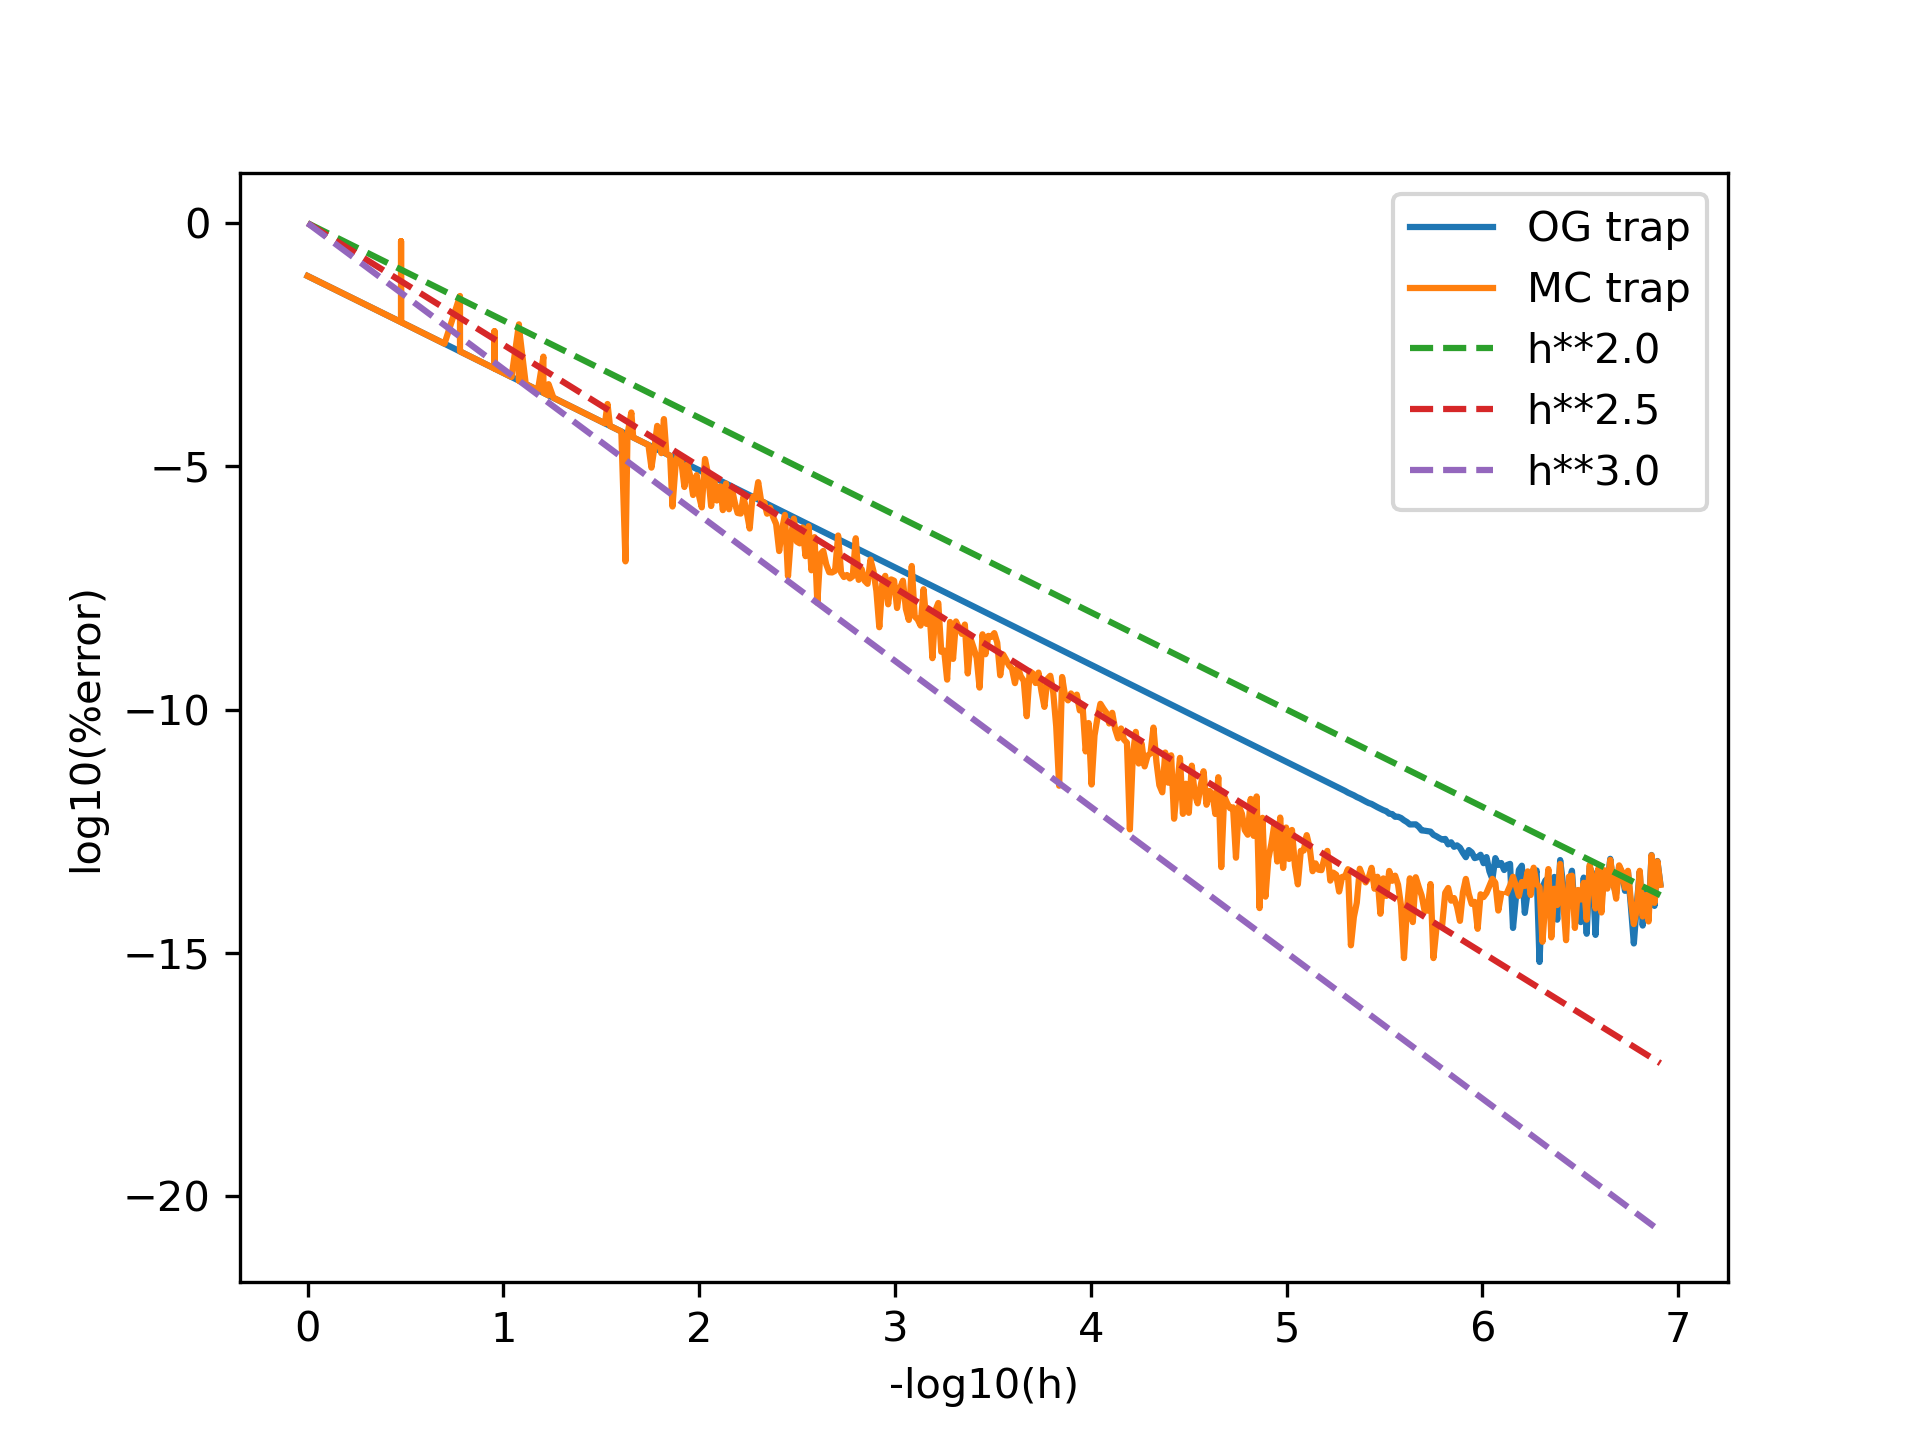
\includegraphics[width=0.8\textwidth]{plots/MCtrap.png}
        \caption{Log-log plot of (\ref{MCtrap}) for
        $\int_{0}^{1}e^{s}ds$ with $l=100$.
        %There are some artifacts of floating-point arithmetic.  
        }
        \label{fig:MCtrap}
    \end{figure}
\end{pythonn}

We postulate that this MC composite rule enhances the convergence
rate by $0.5$ orders compared to the standard composite rule for each dimension,
provided that the appropriate conditions of smoothness are met.
To substantiate this conjecture, we shall outline our rationale concerning
the accumulation of unbiased polynomial errors.\\

For the sake of simplicity, we reduce the study of the local truncation error
to the following expression:
\begin{equation}
    \int_{0}^{h} s^{2}ds = O(h^{3}).
\end{equation}

In the standard composite rule, we would drop this term, but in
the MC version, we eliminate the bias. As a result,
the local truncation error behaves like:

\begin{equation}
    \int_{0}^{h} s^{2}ds- h(hU)^{2} = \int_{0}^{h} s^{2}ds- h^{3}U^{2} = O(h^{3}).
\end{equation}

The main distinction between the standard and MC rule lies in how they
accumulate local truncation errors into global truncation error. In the standard
case, there is a loss of one order. When measuring the error of randomized algorithms
, the root mean square error is typically used, which, in the unbiased case,
is equivalent to the standard deviation:

\begin{align}
    \sqrt{\text{Var}\left(\sum_{j=1}^{n} \int_{0}^{h} s^{2}ds- h^{3}U_{j}^{2}\right)}
     & =\sqrt{\text{Var}\left(\sum_{j=1}^{n} h^{3}U_{j}^{2}\right)}   \\
     & =h^{3} \sqrt{\text{Var}\left( \sum_{j=1}^{n} U_{j}^{2}\right)} \\
     & =h^{3} \sqrt{ \sum_{j=1}^{n}\text{Var} (U_{j}^{2})}            \\
     & =h^{3} \sqrt{ n \text{Var}(U^{2})}                             \\
     & =h^{3} \sqrt{n} \sqrt{ \text{Var}(U^{2})}                      \\
     & = O(h^{2.5}).
\end{align}


\begin{related}
    Optimal theoretical bounds on randomized algorithms can be found in:
    (see literature randomized trapezoidal rule)
    \cite{wu_randomised_2020}. The half order convergence that randomized
    gains over determinstic isn't the same gain we consider.
\end{related}

\subsection{Unbiased Non-Linearity}
In this subsection we introduce techniques to deal with non-linearity.
At first it may looks only possible to deal with linear problems in an unbiased way but by using
independent samples it possible to deal with polynomial non-linearity's (which theoretically extend
to any continuos functions by the Weierstrass approximation theorem).  It is not always easy to
transform non-linearity into polynomials but it is not difficult to come up with
biased alternative approaches based on linearization or approximate polynomial non-linearity.


\begin{example}[$y'=y^{2}$]
    Let's do following example:
    \begin{equation} \label{dyy2}
        y'= y^2,y(1)=-1.
    \end{equation}
    This has solution $-\frac{1}{t}$. Integrate both sides of
    equation (\ref{dyy2}) to arrive at following integral equation:
    \begin{equation} \label{Integral dyy2}
        y(t) = -1 + \int_{1}^{t} y(s) y(s) ds .
    \end{equation}
    To estimate the recursive integral in equation (\ref{Integral ydy}) we use $2$
    independent $Y_{1},Y_{2}\sim Y$ :

    \begin{equation} \label{RRVE yy2}
        Y(t) = -1 + (t-1) Y_{1}(S) Y_{2}(S).
    \end{equation}

    With $S \sim \text{Uniform}(1,t)$. This is a branching RRVE this is
    typical when dealing with non-linearity.
\end{example}

\vspace*{0.2cm}
\begin{pythonn}[$y'=y^{2}$]
    %important note while implementing equation (\ref{RRVE yy2})  
    \pythoncode{python code/dyy2.py}
\end{pythonn}

\begin{example}[$e^{E[X]}$]
    $e^{\int x(s)ds}$ is common expression encountered when studying ODEs.
    In this example we demonstrate how you can generate unbiased estimates of
    $e^{E[X]}$ with simulations of $X$. The taylor series of $e^{x}$ is:
    \begin{align}
        e^{E[X]} & = \sum_{n=0}^{\infty} \frac{E^{n}[X]}{n!}     \\
                 & = 1 + \frac{1}{1}E[X]\left(1+ \frac{1}{2}E[X]
        \left(1+\frac{1}{3}E[X]\left(1+ ...\right)\right)\right). \label{taylor e}
    \end{align}
    Change the fractions of equation (\ref{taylor e}) to Bernoulli processes
    and replace all $X$ with independent $X_j$ with $E[X]=E[X_{i}]$.
    \begin{align}
        e^{E[X]} & = E
        \left[1 + B\left(\frac{1}{1}\right)E[X_1]
        \left(1+ B\left(\frac{1}{2}\right)E[X_2]
        \left(1+B\left(\frac{1}{3}\right)E[X_3]
        \left(1+ ...\right)
        \right)
        \right)
        \right]              \\
                 & = E\left[
            1 + B\left(\frac{1}{1}\right)X_1
            \left(1+ B\left(\frac{1}{2}\right)X_2
            \left(1+B\left(\frac{1}{3}\right)X_3
            \left(1+ ...\right)
            \right)
            \right)
        \right]              \\
    \end{align}
    What is inside the expectation is something that we can simulate with simulations of $X_{j}$.
\end{example}

\vspace{0.2cm}
\begin{pythonn}[$e^{E[X]}$]
    The following python code estimates $e^{\int_{0}^{t} s^{2}ds}$:
    \vspace*{0.4cm}
    \pythoncode{python code/expX.py}
    %}
\end{pythonn}

\begin{related}
    A similar approach to non-linearity can be found in \cite{ermakov_monte_2019}.
    We have more papers on how to deal with non-linearity stashed, no idea if they are
    worth mentioning.
\end{related}

\subsection{Recursion}
In this subsection we discuss recursion related techniques.

\begin{technique}[coupled recursion]
    The idea behind coupled recursion is sharing recursion calls of
    multiple RRVEs for simulation. This does make them dependent.
    It is like assuming $2$ induction hypotheses at the same
    time and proving both inductions steps at the same time vs
    doing separate induction proofs. Which should be easier
    because you have accesses to more assumptions at the same time.
\end{technique}

\begin{example}[coupled recursion] \label{ex:coupled recursion}
    Lets say you are interested in calculating the
    sensitivity of the solution of an ODE to a
    parameter $a$:
    \begin{align}
        y'             & =ay,y(0)=1 \Rightarrow \label{couple recu ex1} \\
        \partial_{a}y' & = y + a \partial_{a}y \label{couple recu ex2}
    \end{align}
    Turn (\ref{couple recu ex1}) and (\ref{couple recu ex2}) into RRVEs.
    To emphasize that they are coupled, that they should
    recurse together we write them in a matrix equation:
    \begin{equation} \label{coupled mat}
        \begin{bmatrix}
            Y(t) \\
            \partial_{a}Y(t)
        \end{bmatrix}=
        X(t)=
        \begin{bmatrix}
            1 \\
            0
        \end{bmatrix}+
        t \begin{bmatrix}
            a & 0 \\
            1 & a
        \end{bmatrix}
        X(Ut).
        % \begin{bmatrix}
        %     Y(Ut) \\
        %     \partial_{a}Y(Ut)
        % \end{bmatrix}.
    \end{equation}
    Notice how this gets rid of the additive branching
    recursion of equation (\ref{couple recu ex2}).

\end{example}

\begin{pythonn} [implementation of (\ref{coupled mat})]
    \pythoncode{python code/coupled_mat.py}
\end{pythonn}

\begin{related}[coupled recursion]
    Example (\ref{ex:coupled recursion}) is inspired by \cite{vicini_path_2021}.
    Coupling feels close to percolation \cite{duminil-copin_sixty_2019}.
\end{related}

\begin{technique}[recursion in recursion]
    Recursion in recursion is what is sounds like. It is like proving an induction
    step of an induction proof with induction.
\end{technique}

%\begin{example}[recursion in recursion]
%    maybe induction in induction proof example or a reference to ODE solvers later.
%\end{example}

\begin{related}[recursion in recursion]
    The next flight variant of WoS
    is a beautiful example of recursion in recursion described in
    \cite{sawhney_grid-free_2022}.
\end{related}

Most programming languages support recursion but this comes with restrictions
like maximum recursion depth and performance issues. When possible tail recursion is
a way to implement recursion that solves those
issues.

\begin{technique}[non-branching tail recursion]
    Tail recursion involves reordering all operations
    so that almost no operation needs to happen after
    the recursion call. This allows us to return the
    answer without retracing all steps when we reach
    the last recursion call, and it can achieve similar
    speeds to a forward implementation.
\end{technique}

The non-branching recursion presented in the RRVEs
can be implemented straightforwardly due to the associativity of
all operations ($(xy)z = x(yz)$) involved. However, tail recursion
may not always be desirable as it discards intermediate values of
the recursion calls which may be of interest. To retain some of these intermediate
values while still partly optimizing for performance, it is possible
to combine tail recursion with normal recursion.

\begin{pythonn}[tail recursion on (\ref{coupled mat})]
    We implement (\ref{coupled mat}) but this time with tail recursion.
    We collect addition operations in a vector $sol$ and multiplication
    in a matrix $W$.
    \vspace{0.3cm}
    \pythoncode{python code/tailrecu.py}
\end{pythonn}

%Branching tail recursion is hard. There  are multiple ways to
%do branching tail recursion with each their advantages and disadvantages. \\
%In the context of recursive MC there are $2$ techniques that
%stand out:

%\begin{technique}[tree regrowing]
%    The structure of branching recursion can be captured by a tree. Storing that tree
%    in memory can be expensive. In recursion you only need to retrace steps
%    $1$ by $1$ therefore you only need local parts of the recursion tree. Tree
%    regrowing tries to alleviate memory issues by instead storing the whole
%    tree only storing seeds (of the random generator) of parts of the
%    tree and growing them when needed.
%\end{technique}
%
%\begin{technique}[backward tail recursion]
%    One way of doing branching tail recursion is by using operation buffers for
%    all leafs which is not memory friendly. In backward tail recursion you retrace
%    steps and do all operations in reverse to recover the buffer needed.
%\end{technique}


\begin{related}[branching recursion]
    This blog discusses branching tail recursion:
    \url{https://jeroenvanwijgerden.me/post/recursion-1/}.
    Interesting techniques  like tail recursion  gets discussed in .
\end{related}


\section{ODEs}

%\subsection{Linear Recursive Integrals}
%We have algo in mind for this case based on coupled recursion on disjunct sets.
%
%\begin{definition}[Volterra equation of the second kind]
%    A Volterra equation of the second kind for $x$  is of the following form:
%    $$
%        x(t)=f(t)+\int_a^t K(t, s) x(s) ds.
%    $$
%    Given the kernel  $K(t, s)$  and  $ f(t)$.
%\end{definition}
%


\subsection{Introduction}
In this subsection we discuss informally how to turn ODEs into integral equations mainly
by example.
Our main tool for this are green functions. Before defining green functions
we do some examples.  \\

\begin{example}[$y'=y$]
    Let's solve
    \begin{equation} \label{ydy int}
        y'=y.
    \end{equation}
    but this time with the following condition:
    \begin{equation}
        \int_{0}^{1} y(s) ds = e-1.
    \end{equation}

    This still has solution $y(t)=e^{t}$. We define the corresponding source
    green function $G(t,x)$ for $y'$ and this type of condition as follows:
    \begin{equation}
        G'= \delta(x-t), \int_{0}^{1}G(s,x)ds = 0.
    \end{equation}
    Solving this obtains:
    \begin{equation}
        G(t,x) = H(t-x) +x-1.
    \end{equation}
    with
    \begin{equation}
        H(x) = \begin{cases}
            0 & \text{ if } x<0 \\
            1 & \text{ else }
        \end{cases}.
    \end{equation}

    Note that we could have used a different green function corresponding
    to a different linear differential operator. \\

    It shouldn't be clear from this point but with this green
    function we form following integral equation for (\ref{ydy int}):
    \begin{equation} \label{int ydy int}
        y(t)= e -1 + \int_{0}^{1}G(t,s)y(s)ds.
    \end{equation}
    Turning equation (\ref{int ydy int}) into a RRVE with recursive MC gives:

    \begin{equation}\label{RRVE ydy int}
        Y(t)= e-1 + 2B\left(\frac{1}{2} \right)Y(S)(H(t-S)+S-1) .
    \end{equation}

    With $S \sim U$. We will be skipping over the python implementation of equation (\ref{RRVE ydy int})
    because it adds nothing new.
    Instead we plot realizations of equation (\ref{RRVE ydy int}) in Figure \ref{fig:ydy int}.

    \begin{figure}[h!]
        \centering
        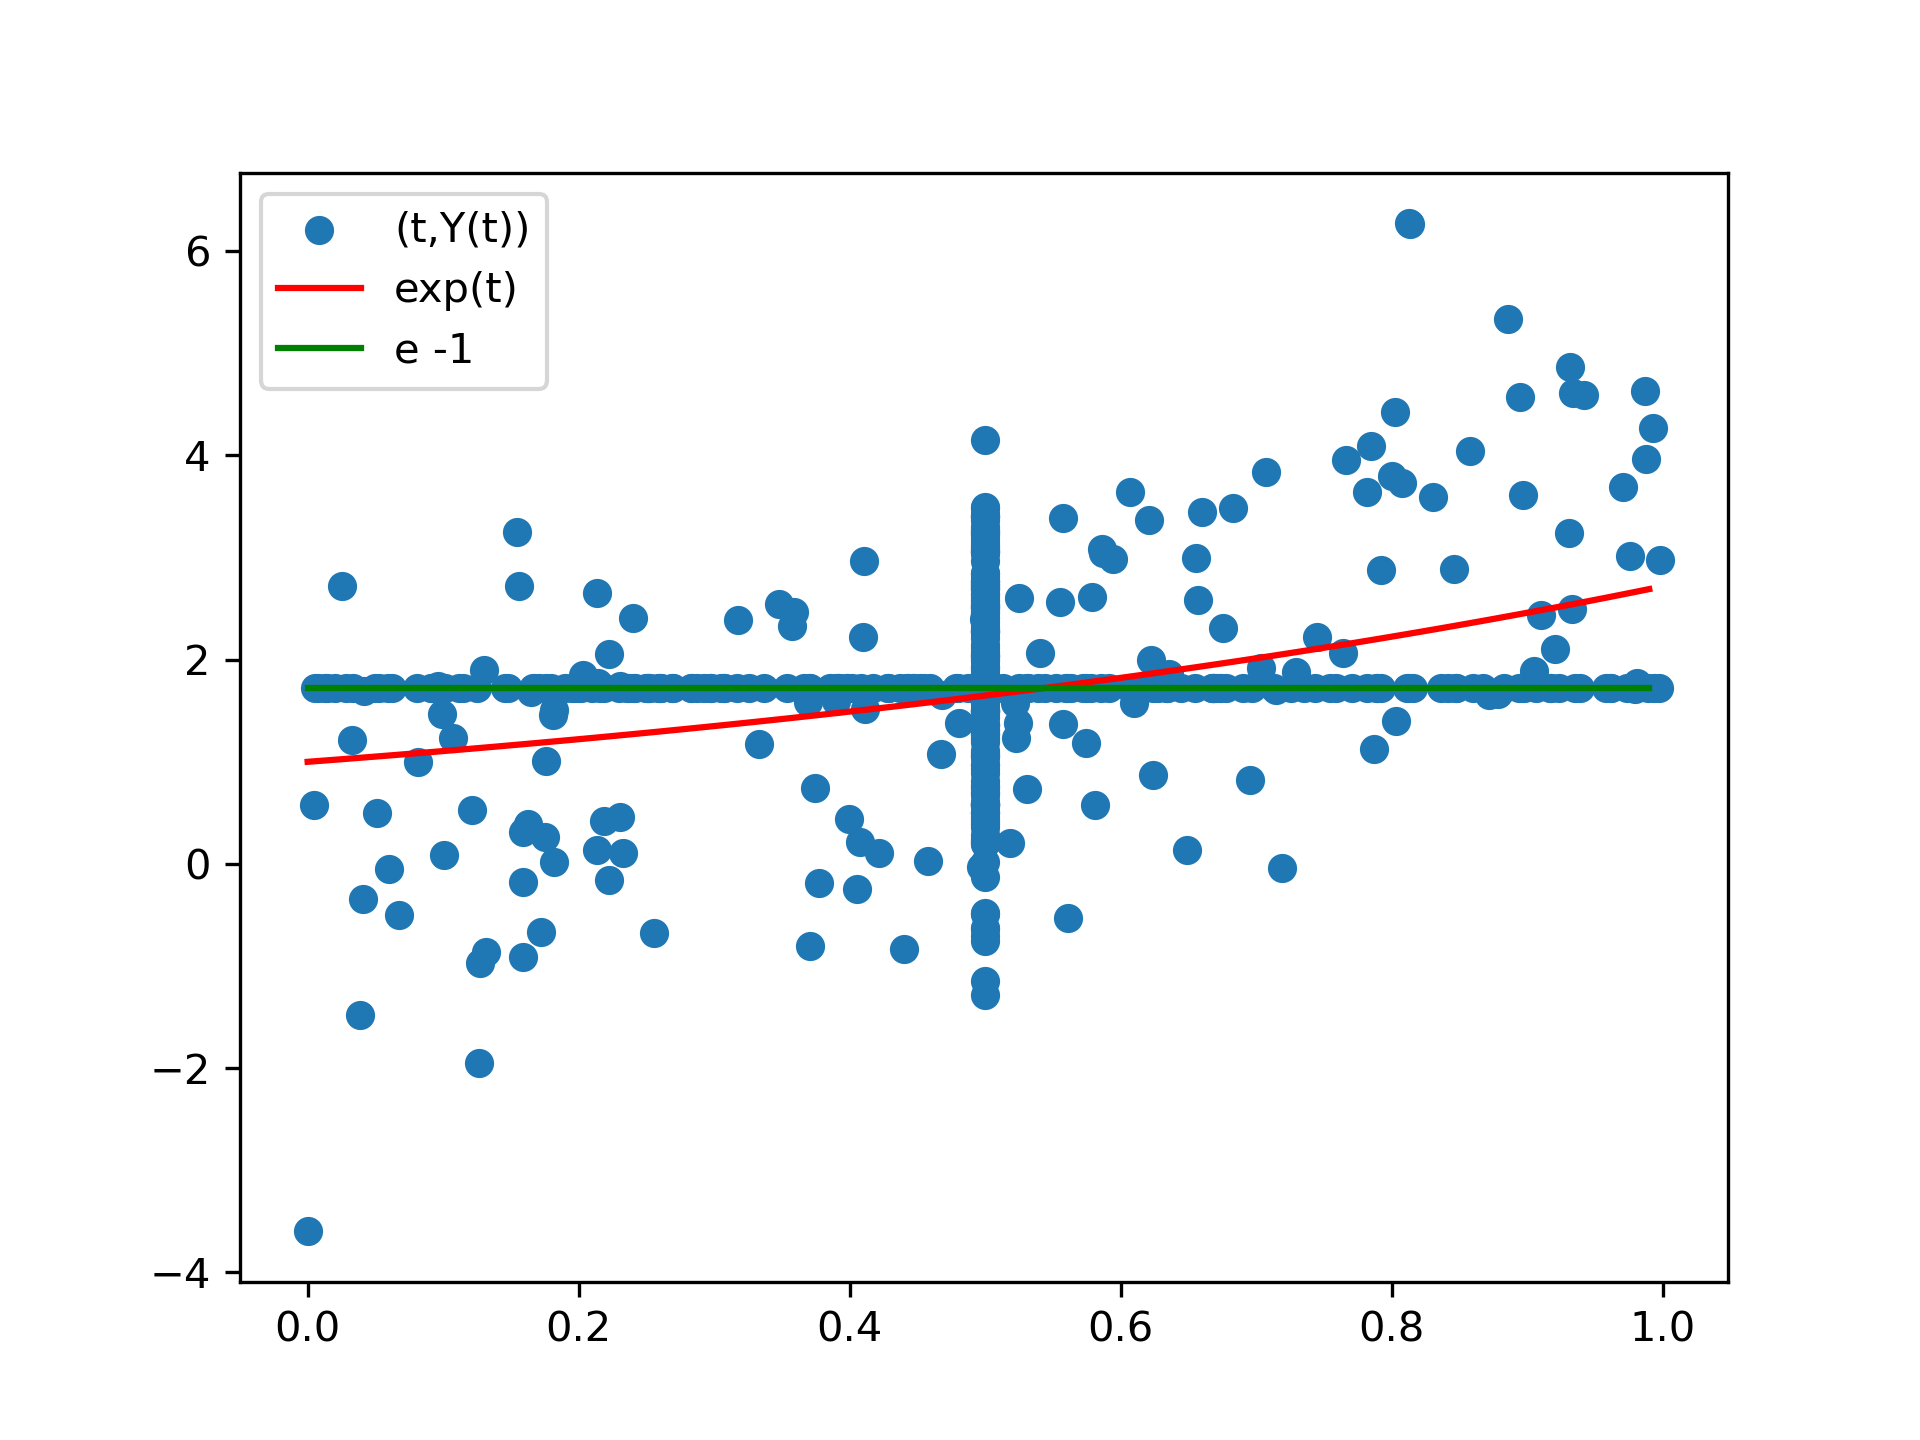
\includegraphics[width=0.8\textwidth]{plots/ydy int.png}
        \caption{Recursive calls of (\ref{RRVE ydy int}) when
            calling $Y(0.5)$ $300$ times. Points accumulate on
            the green line due to the Russian roulette,
            and at  $t=0.5$ because it is the starting
            value of the simulation.
        }
        \label{fig:ydy int}
    \end{figure}

\end{example}

\begin{example}[$y''=y$]
    Lets solve the following boundary problem:
    \begin{equation} \label{ddyy}
        y'' = y, y(0) = 1, y'(1)=e.
    \end{equation}
    This has solution $y(t) = e^{t}$. We define the source green function $G(t,x)$
    for $y''$ and Dirichlet/Neumann boundary conditions in the following way:

    \begin{equation}
        G''= \delta(t-x),G(0)=0,G'(1)=0.
    \end{equation}

    Solving this obtains:

    \begin{equation}
        G(t,x) =
        \begin{cases}
            -t & \text{if } t <  x   \\
            -x & \text{if } t \ge  x
        \end{cases}.
    \end{equation}

    The boundary green function $P(t,x)$ (for $x \in \{0,1\}$)
    for $y''$ and Dirichlet/Neumann boundary conditions is defined
    the following way:
    \begin{equation}
        P'' = 0, \left(P(0,x),P'(1,x) \right)=
        \begin{cases}
            (1 , 0) & \text{ if } x=0 \\
            (0 , 1) & \text{ if } x=1
        \end{cases}.
    \end{equation}

    Which is just a basis for the homogenous solutions for now. Solving
    this gives:

    \begin{equation}
        P(t,x) =
        \begin{cases}
            1 & \text{ if } x=0 \\
            t & \text{ if } x=1
        \end{cases}.
    \end{equation}

    Again it shouldn't be clear from this point but with these set of green
    functions we form following integral equation for (\ref{ddyy}):

    \begin{equation} \label{int ddyy}
        y(t) = P(t,0)y(0) + P(t,1)y(1) + \int_{0}^{1}G(t,s) y(s) ds.
    \end{equation}

    Equation (\ref{int ddyy}) looks like:
    \begin{equation} \label{RRVE ddyy}
        Y(t) = 1 + te + l B\left(\frac{1}{l}\right)G(t,S)Y(S).
    \end{equation}
    With $S \sim U$ and $l>1 \in  \mathbb{R}$. We visualize equation (\ref{RRVE ddyy}) on
    Figure \ref{fig:ddyy}.

    \begin{figure}[h!]
        \centering
        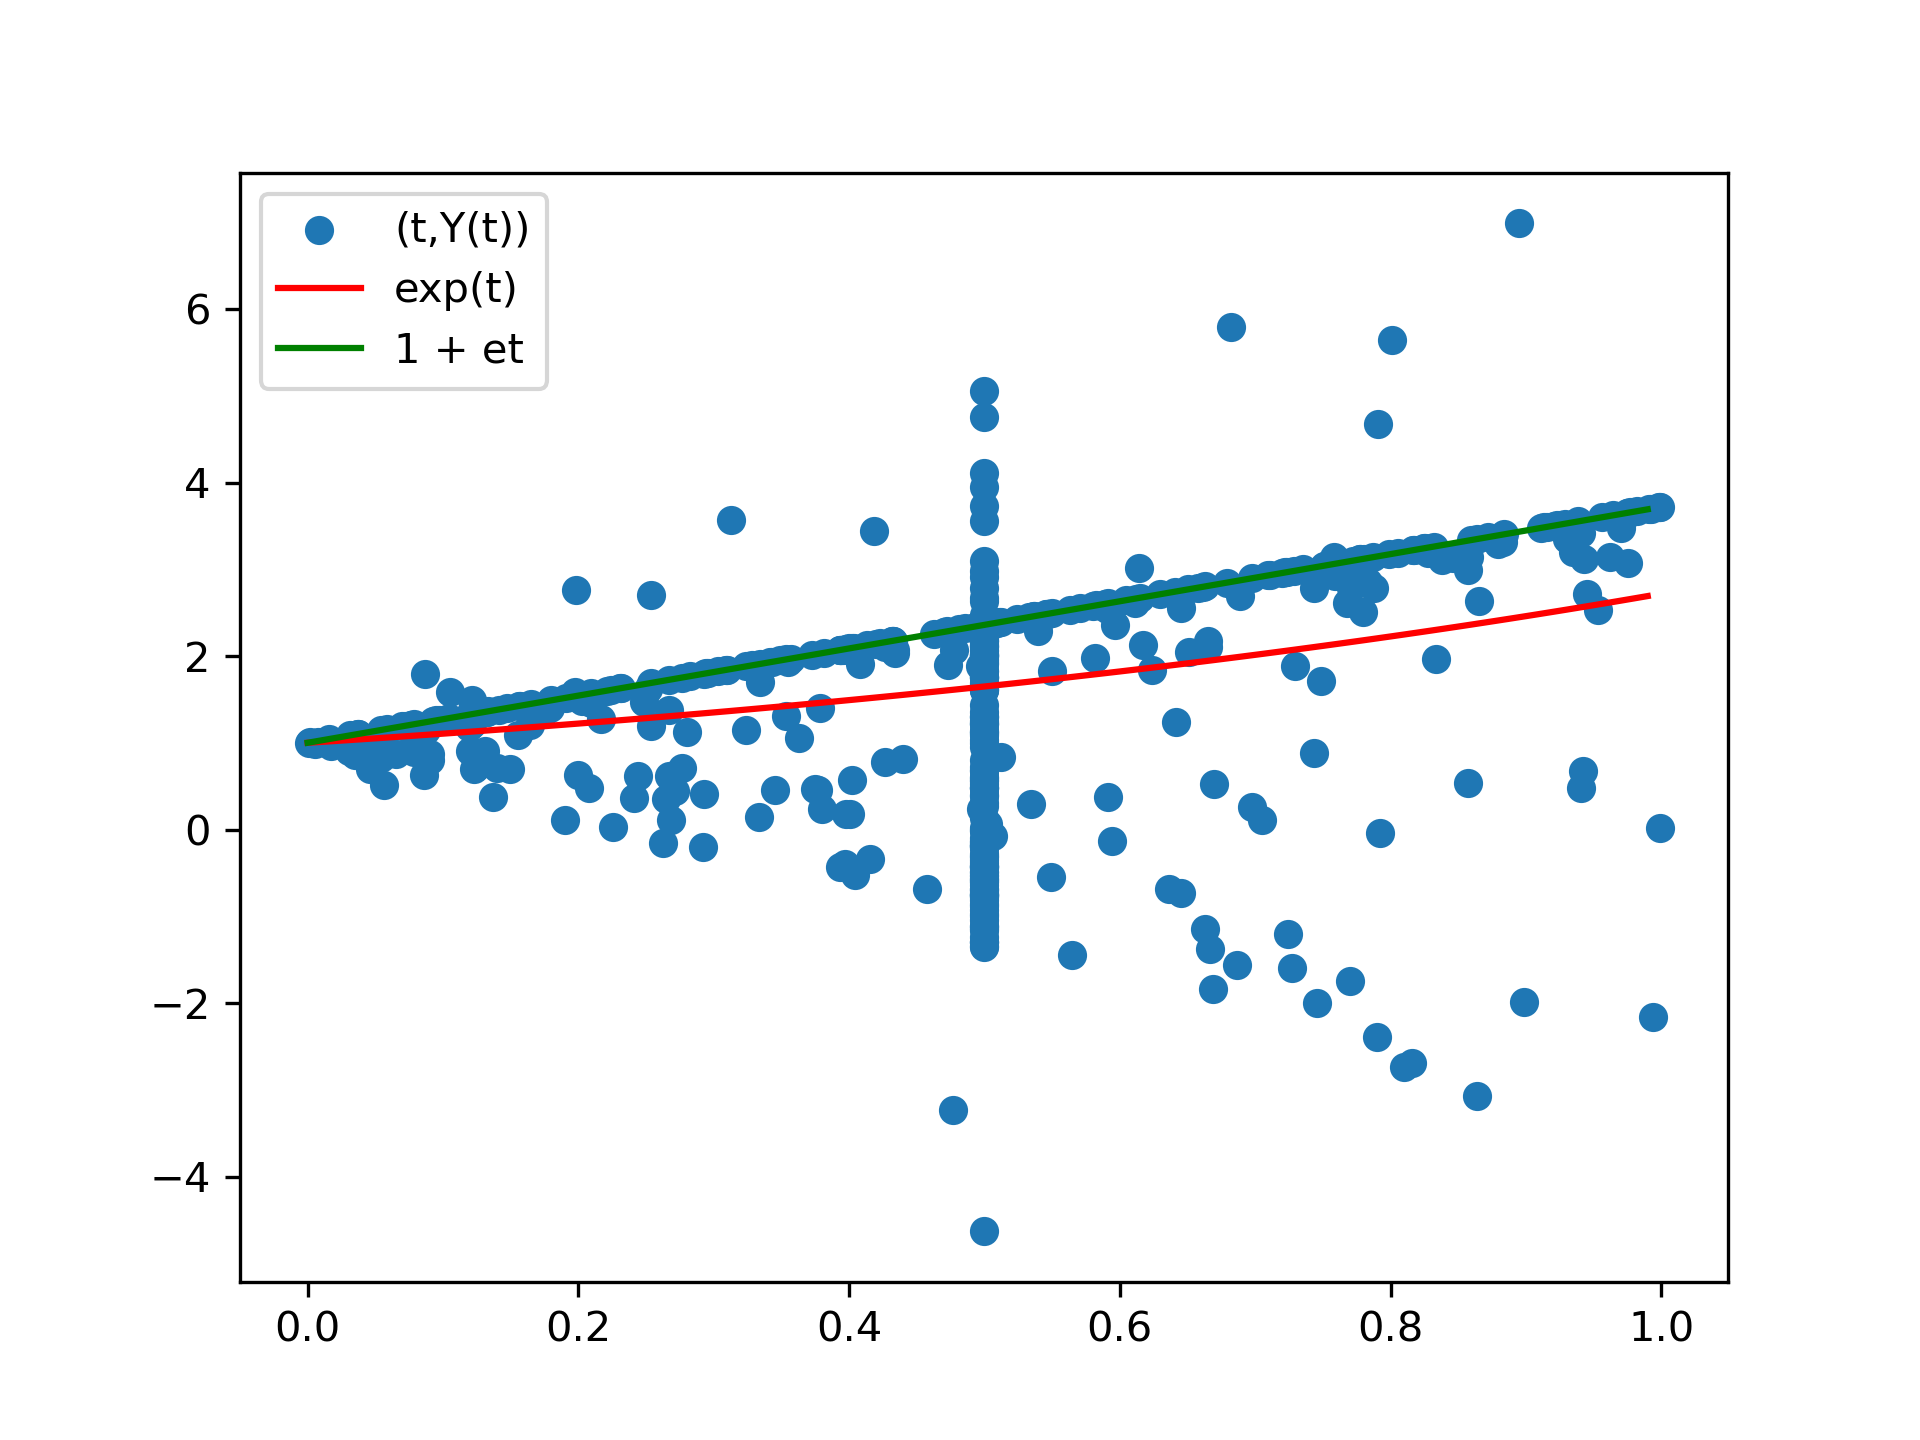
\includegraphics[width=0.8\textwidth]{plots/ddyy.png}
        \caption{Recursive calls of (\ref{RRVE ddyy}), $l=2$ when
            calling $Y(0.5)$ $300$ times.}
        \label{fig:ddyy}
    \end{figure}

\end{example}


%\begin{definition}[boundary green function]
%    we write this later
%    %   The boundary green function of a linear differential problem with linear boundary
%    %   conditions.
%\end{definition}
%
%\begin{definition}[source green function]
%    we write this later
%    %    For
%    %    \[
%    %        L(y(z)) = f
%    %        .\]
%    %    with $L$ a linear differential operator, $z$ a point in the input space of $y$
%    %    ,$f$ arbitrary and linear boundary conditions.
%    %    We define the source green function $G(z,s)$ with following property
%    %    \[
%    %        L(G(z,s))=\delta(z-s).
%    %        .\C
%    %    and null boundary conditions.
%\end{definition}
%
%
%\begin{example}[numerical green functions]
%    There will be probably some green functions that we need
%    that don't have an analytic expression yet.
%\end{example}

% Green's function vs green function (check chatgpt for the answer)
\begin{definition}[green function]
    Vaguely speaking we define the green function as a type of kernel function that we use
    to solve linear problems with linear conditions. The Green's function is the kernel that
    we need to put in front of  the linear conditions or the source term that we integrate
    over and to obtain the solution  and the green function has the property that it satisfies
    either null linear conditions and a Dirac delta source term, or vice versa.
\end{definition}

\begin{related}[green function]
    Our notion of green function is similar to that in \cite{hwang_simulationtabulation_2001}.
\end{related}

% maybe an example of difference equation

\subsection{Convergence}
% \subsection{Fredholm equations}

The ODE examples we have seen so far exhibit rapidly increasing variance as the domain increases,
some cases this leads to non-convergence. However, we have not yet discussed convergence
criteria for recursive Monte Carlo. Rather than delving deeply into variance
or convergence analysis, we will suggest potential solutions in this subsection.

\begin{example}[Dirichlet $y''=y$] \label{main dirichlet}
    The following problem will be the main testing example for
    boundary value problems:
    \begin{equation} \label{eq:main dirichlet}
        y''=y, y(b_{0}),y(b_{1}).
    \end{equation}
    The green functions corresponding to $y''$ and Dirichlet conditions are:

    \begin{align}
        P(t,x) & = \begin{cases}
                       \frac{b_{1}-t}{b_{1}-b_{0}} & \text{if } x = b_{0} \\
                       \frac{t-b_{0}}{b_{1}-b_{0}} & \text{if } x = b_{1}
                   \end{cases}       \\
        G(t,s) & = \begin{cases}
                       -\frac{(b_{1}-t)(s-b_{0})}{b_{1}-b_{0}} & \text{if } s<t \\
                       -\frac{(b_{1}-s)(t-b_{0})}{b_{1}-b_{0}} & \text{if } t<s
                   \end{cases}.
    \end{align}
    Straight from these green functions you get following integral equation and RRVE:
    \begin{align} \label{inteq:main dirichlet}
        y(t) & = P(t,b_{0}) y(b_{0}) + P(t,b_{1}) y(b_{1}) + \int_{b_{0}}^{b_{1}} G(t,s)y(s) ds \\
        Y(t) & = P(t,b_{0}) y(b_{0}) + P(t,b_{1}) y(b_{1})
        + l B\left(\frac{1}{l} \right)(b_{1}-b_{0}) G(t,S)y(S) . \label{RRVE:main dirichlet}
    \end{align}
    With $l \in \mathbb{R}$ the Russian roulette rate and $S \sim \text{Uniform}(b_{1},b_{0})$.

\end{example}

\begin{figure}[h!]
    \centering
    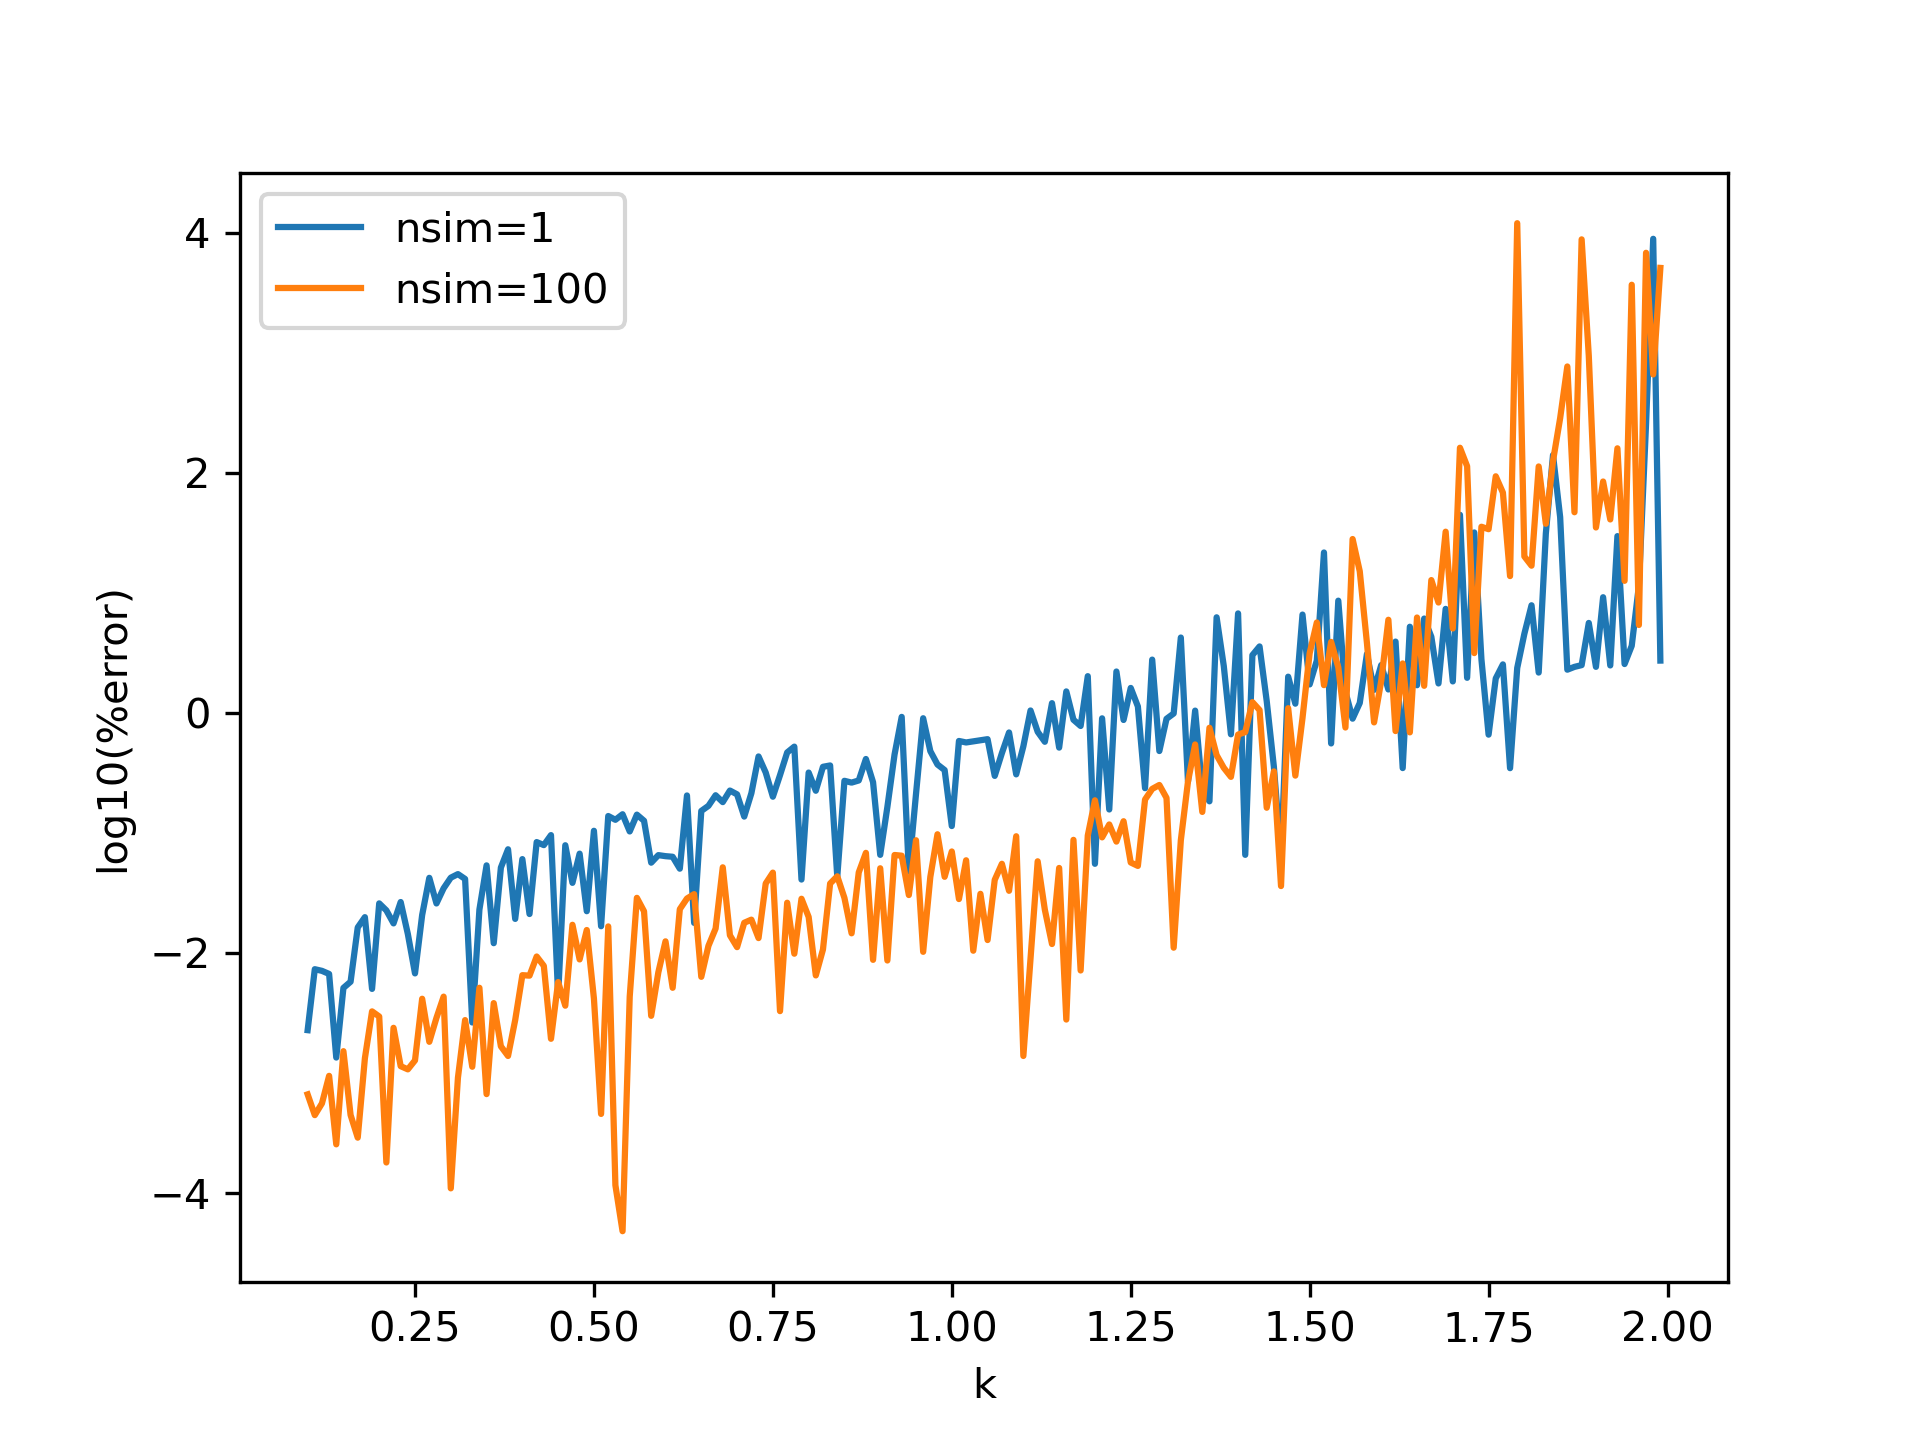
\includegraphics[width=0.8\textwidth]{plots/mainD explosion.png}
    \caption{The logarithmic percentage error of $Y(0)$ for
    (\ref{RRVE:main dirichlet}), with $l=1.2$ and initial conditions
    $y(-k)=e^{-k}$ and $y(k)=e^{k}$, displays an exponential
    increase until approximately $k=1.5$, beyond which additional
    simulations fail to reduce the error, indicating that the variance
    doesn't exist.}
    \label{fig:mainD explosion}
\end{figure}

\begin{definition}[Fredholm equation of the second kind]
    A Fredholm equation of the second kind for $\varphi$  is of the following form:
    \begin{equation}
        \varphi(t)=f(t)+\lambda \int_a^b K(t, s) \varphi(s) ds.
    \end{equation}
    Given the kernel  $K(t, s)$  and  $ f(t)$.
\end{definition}

% comes straight from wikipedia
% \begin{definition}[Liouville–Neumann series]
%     The Liouville–Neumann series for a Fredholm equation of the second kind
%     is defined as
%     \begin{equation}
%         \phi(x)=\sum_{n=0}^{\infty} \lambda^n \phi_n(x).
%     \end{equation}

%     If the $n$th iterated kernel is defined as $n-1$ nested integrals of $n$ operators $K$,

%     $$
%         K_n(x, z)=\iint \cdots \int K\left(x, y_1\right) K\left(y_1, y_2\right)
%         \cdots K\left(y_{n-1}, z\right) d y_1 d y_2 \cdots d y_{n-1}
%     $$
%     $K_0$ may be taken to be $\delta(x-z)$.

%     then

%     $$
%         \phi_n(x)=\int K_n(x, z) f(z) d z
%     $$

%     With

%     $$
%         \phi_0(x)=f(x),
%     $$

%     so
% \end{definition}


% fix point argument is when von neumann series converges

If both $K$ and $f$ are nice, then for sufficiently small $\lambda$,
it is straightforward to establish the existence and uniqueness of solutions
for Fredholm equations of the second kind using a fix point argument. \\


We would like to have MC algorithm that converges in that case. Our best guess is
a combination of splitting and coupling.


\begin{example}[coupled splitting on (\ref{main dirichlet})] \label{ex:coupled splitting}
    Next to normal splitting (\ref{def:splitting}) we can
    also split the domain in equation (\ref{inteq:main dirichlet}):
    \begin{align}\label{inteq:coupled splitting}
        y(t) & = P(t,b_{0}) y(b_{0}) + P(t,b_{1}) y(b_{1}) +
        \frac{1}{2} \int_{b_{0}}^{b_{1}} G(t,s)y(s) ds +
        \frac{1}{2} \int_{b_{0}}^{b_{1}} G(t,s)y(s) ds                                              \\
        y(t) & = P(t,b_{0}) y(b_{0}) + P(t,b_{1}) y(b_{1}) + \label{inteq:coupled domain splitting}
        \int_{b_{0}}^{\frac{b_{1}+b_{0}}{2}} G(t,s)y(s) ds +
        \int_{\frac{b_{1}+b_{0}}{2}}^{b_{1}} G(t,s)y(s) ds
    \end{align}

    Coupling can get rid of the additive branching recursion in the RRVEs corresponding
    to (\ref{inteq:coupled splitting}) and (\ref{inteq:coupled domain splitting}).
    Resulting in following RRVE:
    \begin{equation} \label{RRVE:coupled splitting}
        X(t_{1},t_{2})=
        \begin{bmatrix}
            P(t_{1},b_{0}) & P(t_{1},b_{1}) \\
            P(t_{2},b_{0}) & P(t_{2},b_{1})
        \end{bmatrix}
        \begin{bmatrix}
            y(b_{0}) \\
            y(b_{1})
        \end{bmatrix}
        +
        W
        \begin{bmatrix}
            G(t_{1},S_{1}) & G(t_{1},S_{2}) \\
            G(t_{2},S_{1}) & G(t_{2},S_{2})
        \end{bmatrix}
        X(S_{1},S_{2}).
    \end{equation}
    With $W$ the right weighting matrix (see code (\ref{py:coupled splitting}) for an example)
    and $S_{1},S_{2}$ can be chosen in various ways.
\end{example}

\begin{pythonn}[implementation of (\ref{RRVE:coupled splitting})] \label{py:coupled splitting}
    We implemented equation (\ref{RRVE:coupled splitting}) in example
    (\ref{ex:coupled splitting}) with recursion but in this case it
    is actually possible to implement it forwardly because the time
    proces is nice. \\
    \pythoncode{python code/coupled_splitting.py}

    % can probably make a better plot then this one
    \begin{figure}[h!]
        \centering
        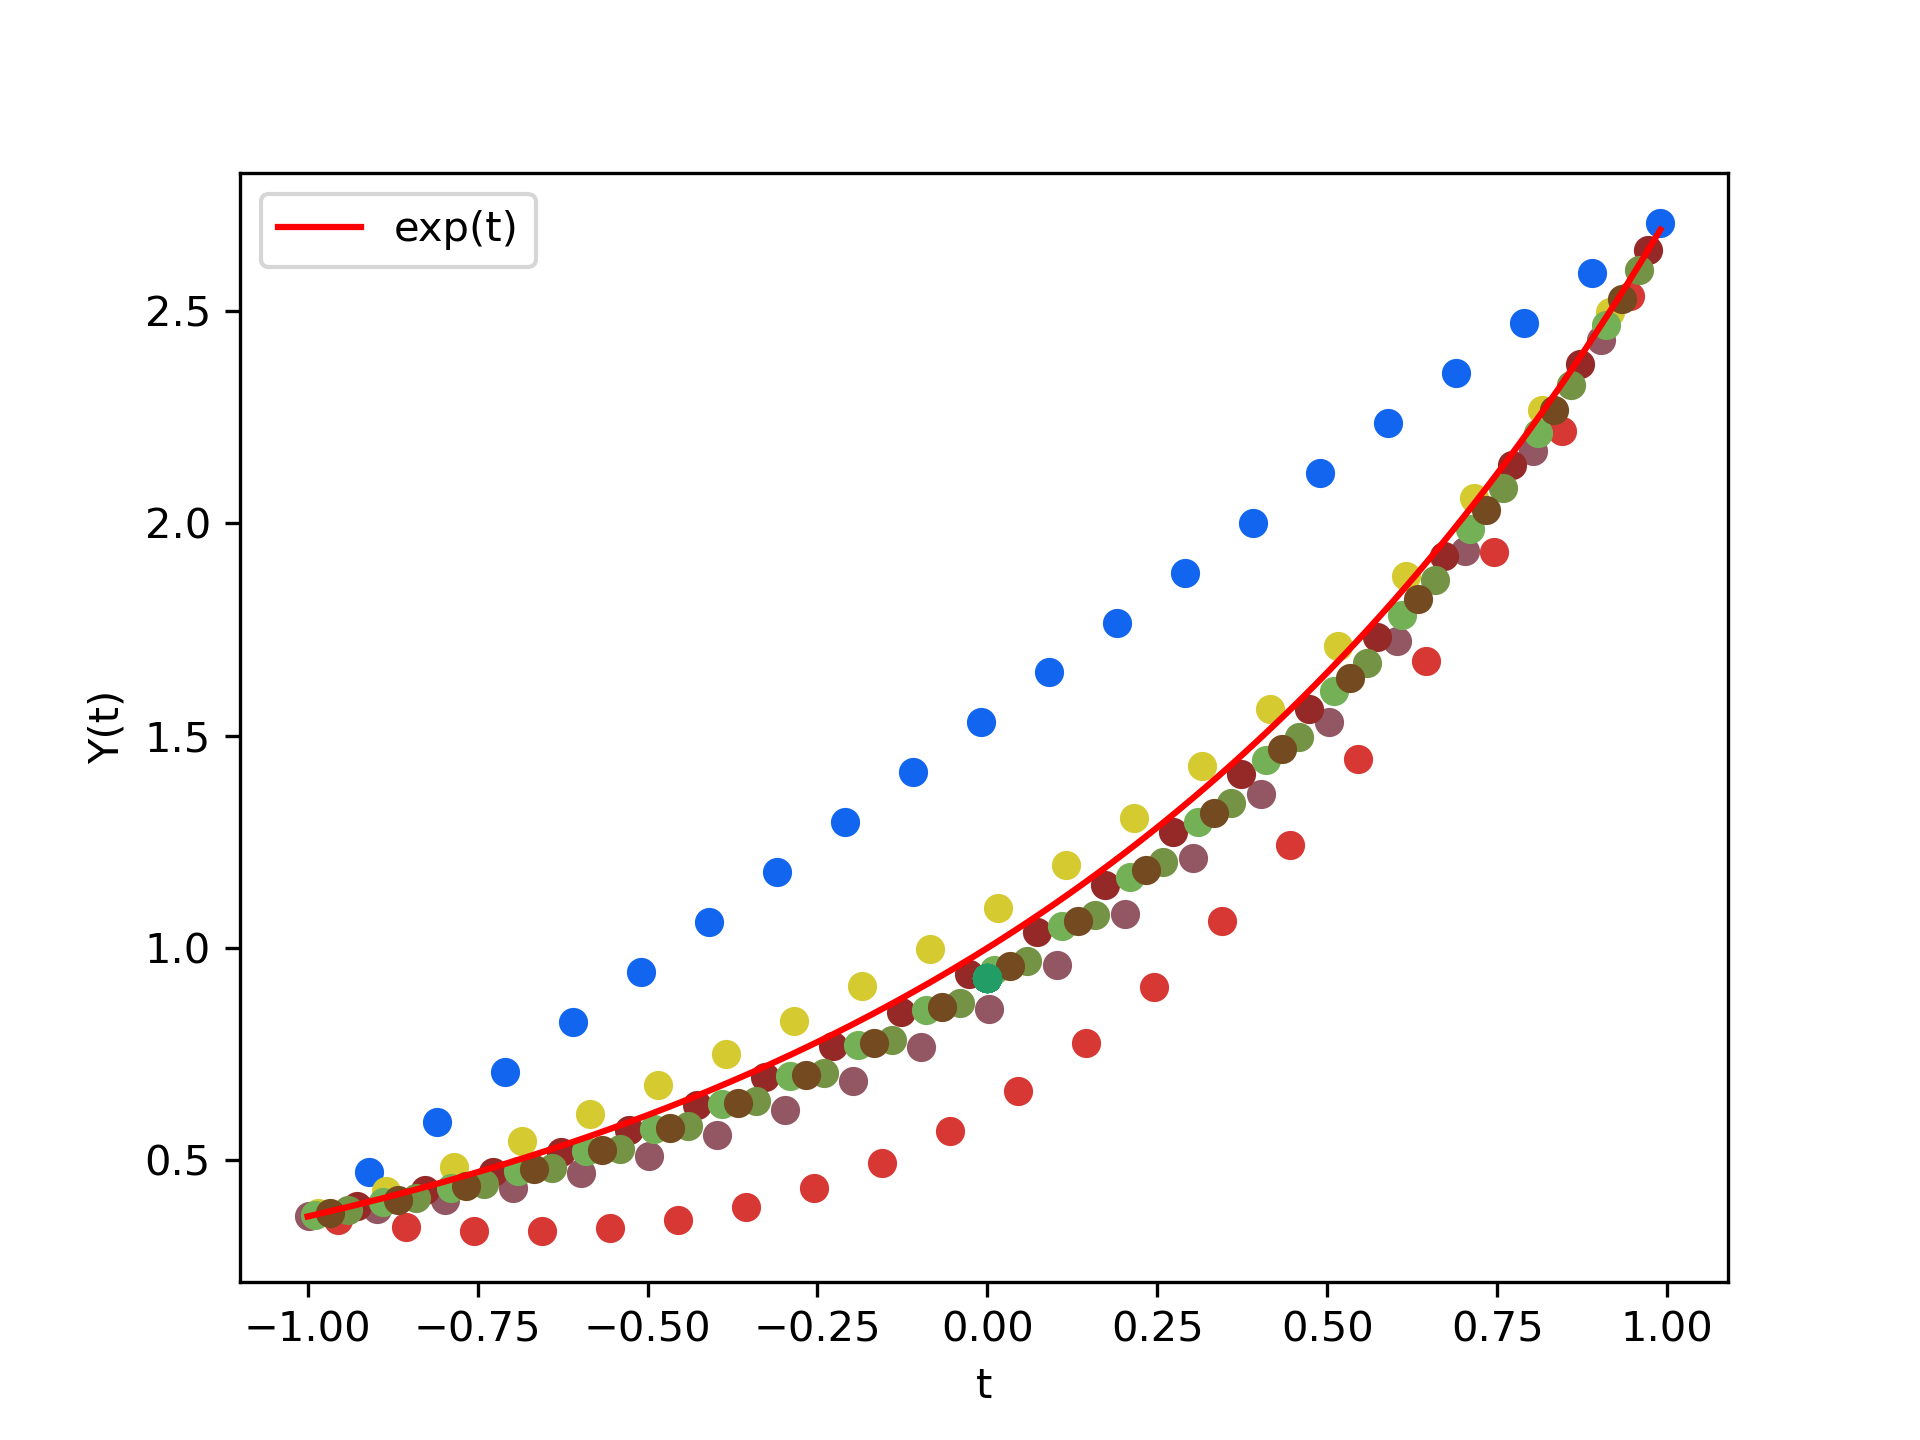
\includegraphics[width=0.8\textwidth]{plots/coupled split.png}
        \caption{Recursive calls of equation (\ref{RRVE:coupled splitting}) when
        calling $X(0)$ once,
        with a split size of $20$, $S_{j}$ coupled such
        they're equally spaced (they don't have to be independent) and coupling is colored.
        The initial conditions for this call are $y(-1)=e^{-1}$ and $y(1)=e^{1}$,
        with Russian roulette rate $l=1.2$.  }
        \label{fig:coupled splitting}
    \end{figure}
\end{pythonn}


It appears that  Figure \ref{fig:coupled splitting}
resemble a fixed point iterations, leading us to hypothesize
that coupled splitting can achieve convergence in most cases
where a fixed point argument holds true. \\

We also conjecture that the convergence speed is very similar
to fix points methods until the accuracy of the stochastic
approximation of the operator is reached (which is the most important
bottleneck). A way around this
is by increasing coupled splitting amount  when reaching this bottleneck
which can be done very straightforward,
making it similar to a multi-grid method. Alternatively when reaching
the bottleneck it is possible to rely on MC convergence.
% (Additional
% iterations beyond the bottleneck do not
% bring the solution closer but they still remain unbiased with low variance)
\\

Coupled splitting was tested on the example shown in Figure
\ref{fig:mainD explosion}, but it did not contribute to the
convergence of the method. This suggests that a fix point argument
would not be effective for this particular example with this
Russian roulette. \\

\begin{related}[coupled splitting]
    Similar ideas to coupled splitting gets discussed in
    \cite{sabelfeld_sparsified_2009}. (the paper on using more rows
    for MC in linear systems) \\

    Example (\ref{ex:coupled splitting}) is not the best example to demonstrate
    coupled splitting. First the problem is local and second everything is smooth.
    Later we discuss algorithms that abuse locality via recursion in recursion and
    smoothness with control variates. A better use case for this algorithm is for
    Fredholm equations of the second kind with for example a non-smooth kernel or
    a nasty domain.
    Similar use cases for MC in differential equations get discussed in
    \cite{jentzen_random_2009}. \\

    See \cite{gupta_convergence_2021} for a discussion on convergence
    of recursive stochastic algorithms.
\end{related}

% explaining that coupled split is cool for global problems but for
% ODEs and PDEs we are interested in exploiting locality.

\subsection{IVPs ODEs}
In this subsection we do some IVPs examples. \\

Right now we don't have a general RMC algorithm that can
guarantee a reasonable variance when increasing the time domain.
Classing IVP solvers rely on shrinking the time steps for
convergence. Recursion in Recursion MC (RRMC) for IVPs tries to emulate
this behavior.

\begin{example}[RRMC $y'=y$] \label{ex:RRMC IVP}
    Let's us explain RRMC for IVPs with our main example.
    Imagine we have a time stepping sheme $(t_{n})$ ($t_{n}> t_{n-1}$)
    then following integral equations hold:
    \begin{equation}
        y(t)= y(t_{n}) + \int_{t_{n}}^{t}y(s)ds , t>t_{n}.
    \end{equation}
    Turn these in following class of RRVEs:

    \begin{equation}
        Y_{n}(t) = y(t_{n}) + (t-t_{n})Y_{n}((t-t_{n})U+t_{n}), t>t_{n}.
    \end{equation}

    A problem with these RRVEs is that we don't know $y(t_{n})$.
    Instead we can replace it with an unbiased estimate $y_{n}$
    which we keep frozen:
    \begin{align}
        \label{eq:RRMC IVP inner}
        Y_{n}(t) & = y_{n} + (t-t_{n})Y_{n}((t-t_{n})U+t_{n}), t>t_{n} \\
        y_{n}    & = \begin{cases}
                         Y_{n-1}(t_{n}) & \text{ if } n \neq 0 \\
                         y(t_{0})       & \text{ if } n = 0
                     \end{cases}.
        \label{eq:RRMC IVP outer}
    \end{align}
    We refer to equation (\ref{eq:RRMC IVP inner}) as the inner recursion and
    equation (\ref{eq:RRMC IVP outer}) as the outer recursion of the recursion in
    recursion.
\end{example}
% maybe measurements of amount of calls to f

\begin{pythonn}[implementation of (\ref{ex:RRMC IVP})] \label{py:RRMC IVP}
    \pythoncode{python code/RRMC_IVP.py}
    We measured the convergence speed to be $O\left(\frac{h^{1.5}}{\sqrt{\text{nsim}}}
        \right)$.

    \begin{figure}[h!]
        \centering
        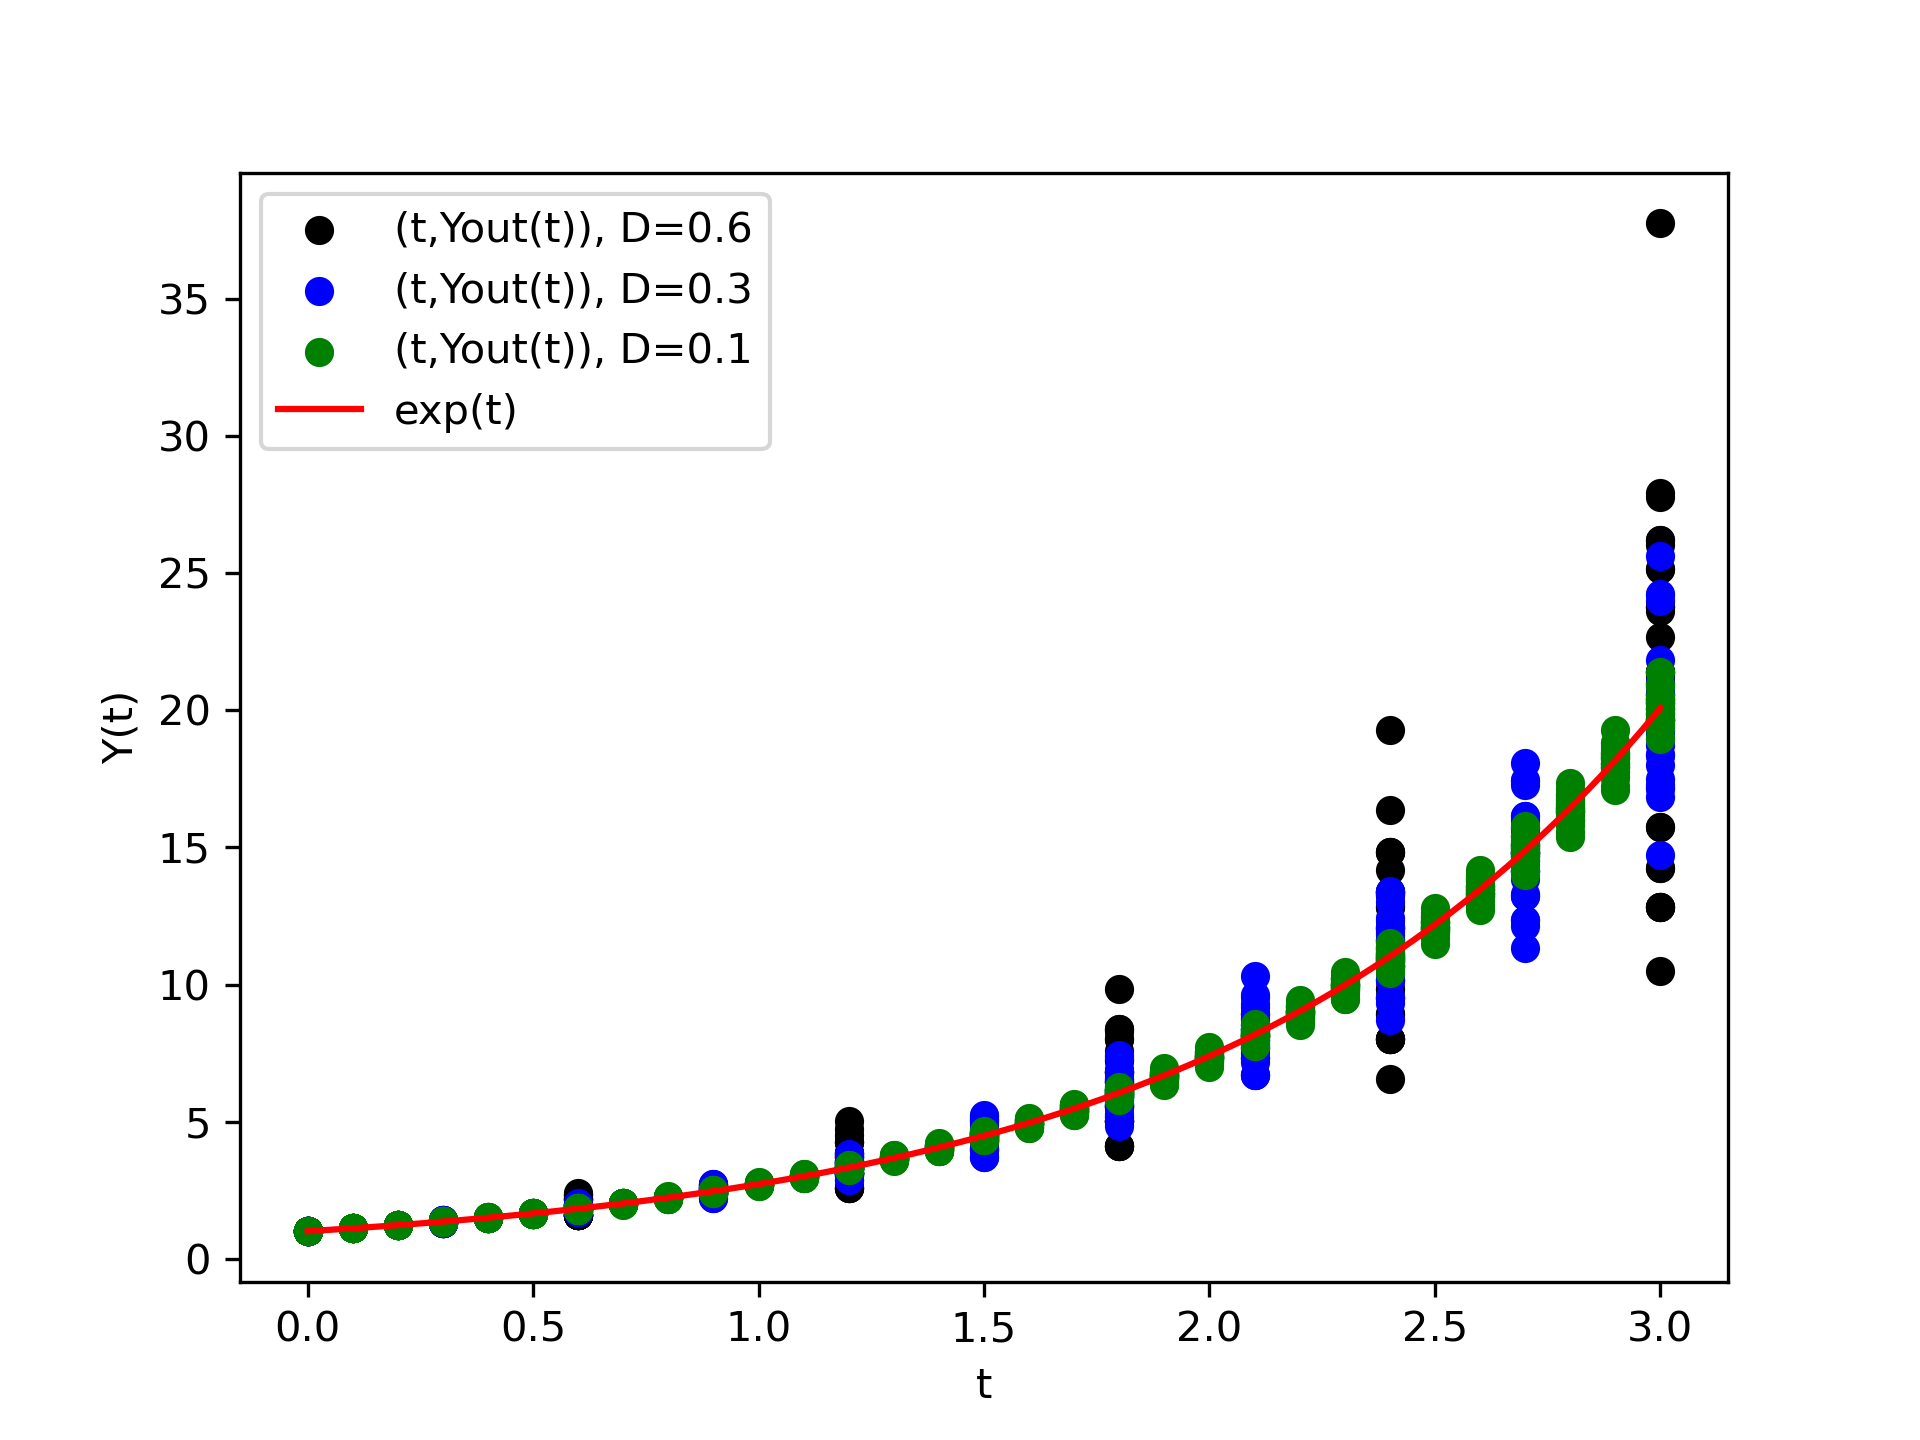
\includegraphics[width=0.8\textwidth]{plots/RRMC IVP.png}
        \caption{Recursive calls of equation (\ref{eq:RRMC IVP outer})
            when calling $Y_{\text{out}}(3,h)$ $30$ times for different $h$.  }
        \label{fig:RRMC IVP}
    \end{figure}
\end{pythonn}

$1.5$ order of convergence is cool but this begs the question on how to achieve
higher order of convergence in $h$. Again it is easy to imitate classical methods
to achieve higher order convergence. We do this by removing lower order terms (which requires
smoothness) with control variates like the MC trapezoidal rule (\ref{MCtrap}).

\begin{example}[CV RRMC $y'=y$]\label{ex:CV RRMC IVP}
    Let us control variate example (\ref{ex:RRMC IVP}). Start
    with:
    \begin{equation}
        y(t)= y(t_{n}) + \int_{t_{n}}^{t}y(s)ds , t>t_{n}.
    \end{equation}
    We need a lower order approximation of the integrand:
    \begin{align}
        y(s) & = y(t_{n}) + (s-t_{n})y'(t_{n}) + O((s-t_{n})^{2})       \\
             & \approx y(t_{n}) + (s-t_{n})f(y(t_{n}),t_{n})            \\
             & \approx y(t_{n}) +
        (s-t_{n})\left(\frac{y(t_{n})-y(t_{n-1})}{t_{n}-t_{n-1}}\right) \\
             & \approx y(t_{n})(1+s-t_{n}).
    \end{align}

    Using the last one as a control variate for the integral:
    \begin{align}
        y(t) & = y(t_{n}) + \int_{t_{n}}^{t}y(s)ds                                          \\
             & = y(t_{n}) + \int_{t_{n}}^{t}y(s)-y(t_{n})(1+s-t_{n}) +y(t_{n})(1+s-t_{n})ds \\
             & = y(t_{n})\left(1 + (1-t_{n})(t-t_{n})+\frac{t^{2}-t_{n}^{2}}{2}\right)
        + \int_{t_{n}}^{t}y(s)-y(t_{n})(1+s-t_{n})ds.
    \end{align}
    We won't discuss turning this into an RRVE nor the implementation. The implementation
    is very similar to (\ref{py:nonlinear RRMC IVP}) and
    Figure \ref{fig:CV RRMC IVP} is a convergence plot for this example.

    \begin{figure}[h!]
        \centering
        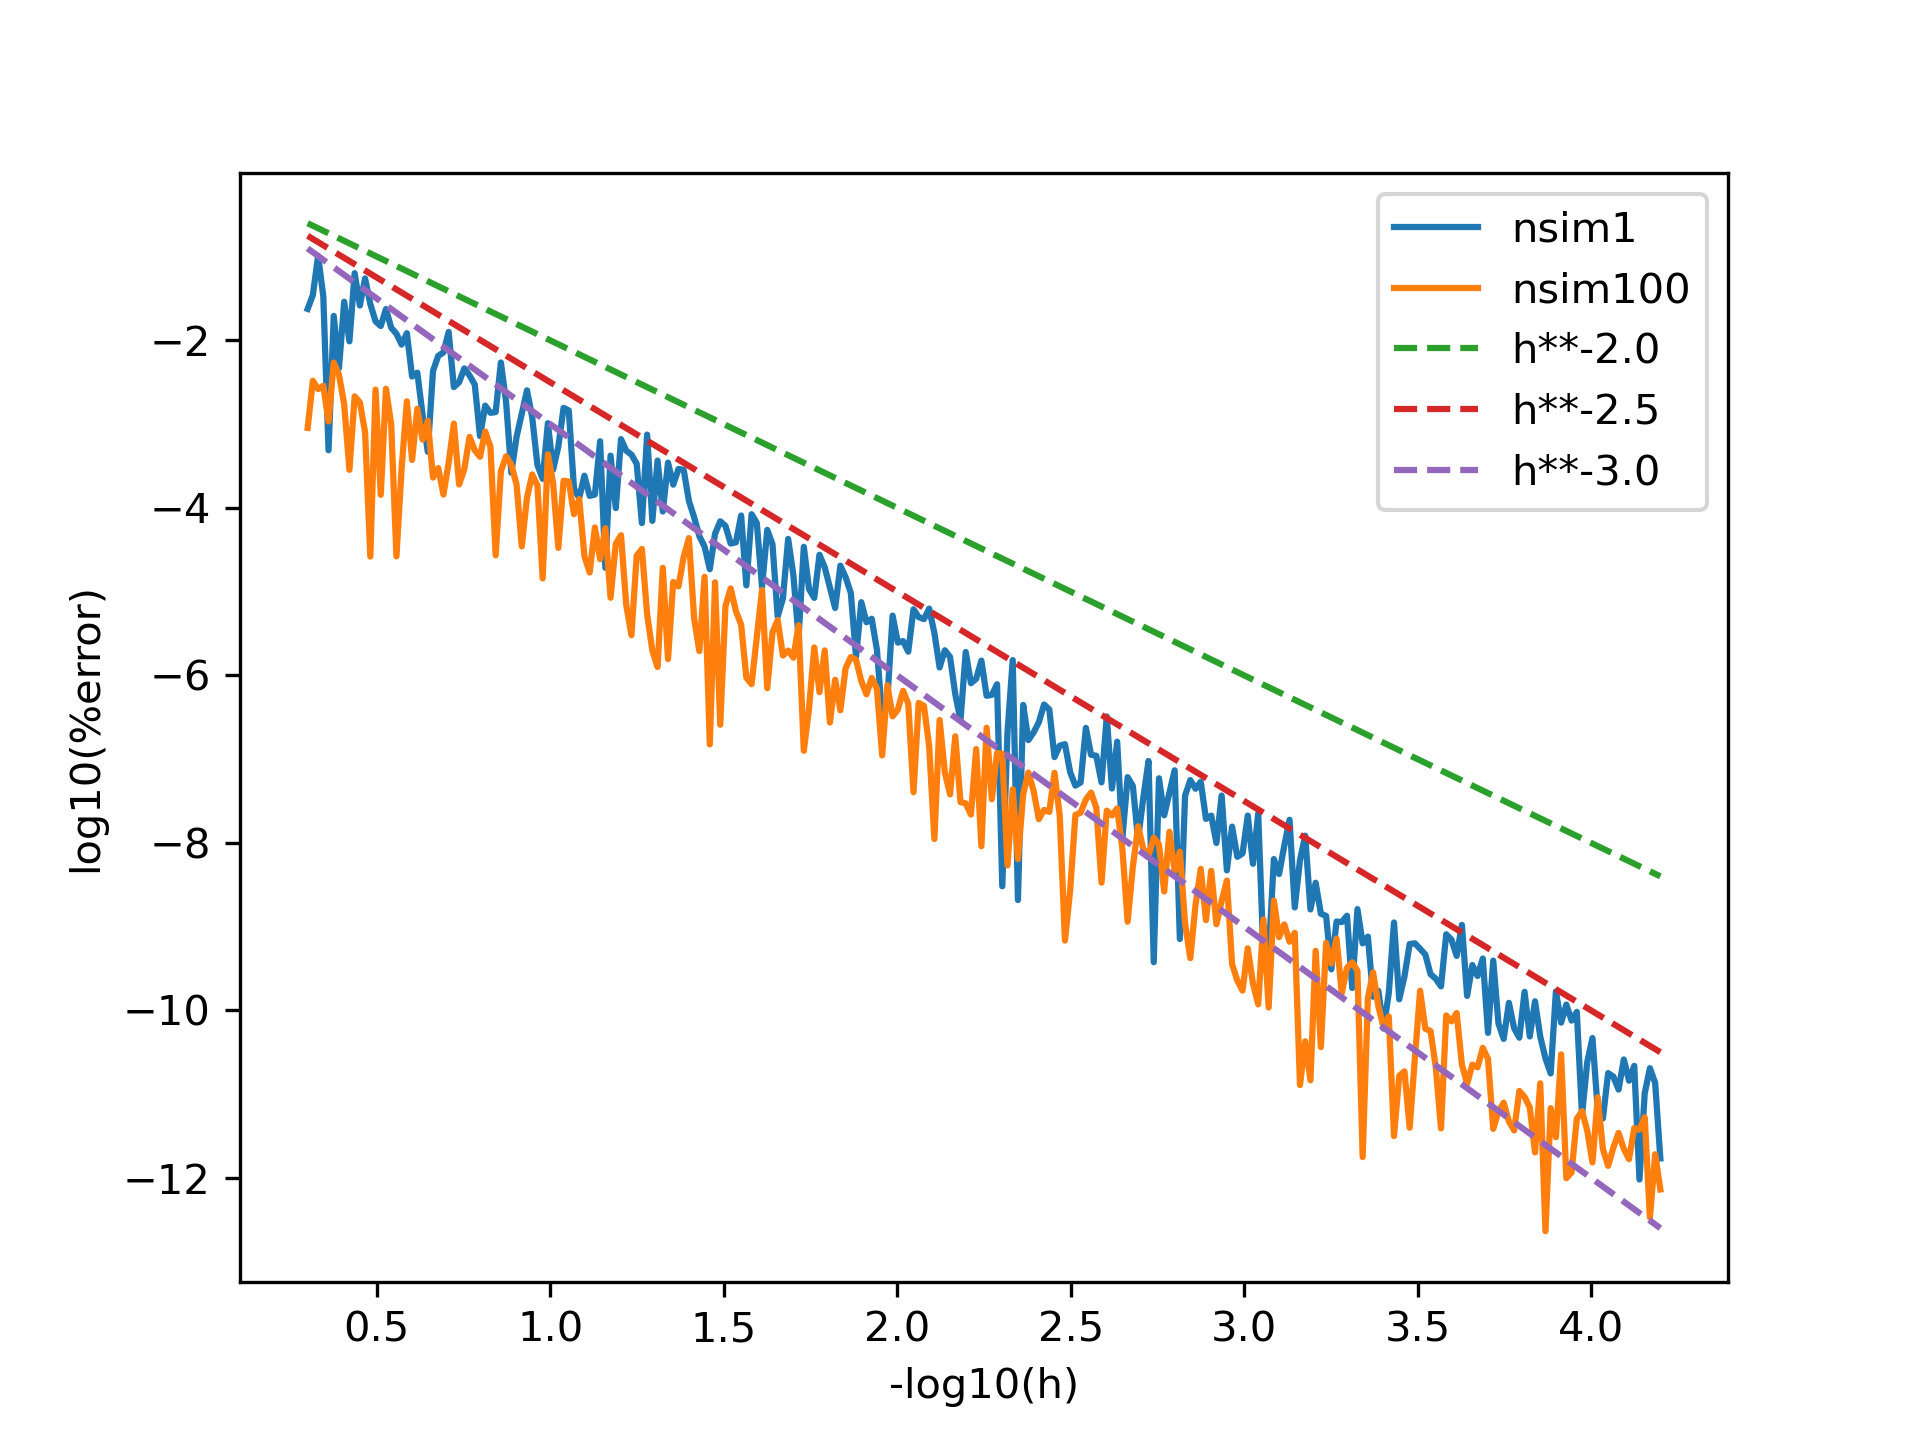
\includegraphics[width=0.8\textwidth]{plots/CV RRMC IVP.png}
        \caption{Log-log plot of example (\ref{ex:CV RRMC IVP}).}
        \label{fig:CV RRMC IVP}
    \end{figure}
\end{example}

\begin{related}[CV RRMC]
    \cite{daun_randomized_2011} also uses control variates to achieve
    a higher order of convergence.
\end{related}

RRMC is biased for our approach to non-linear problems.
The inner recursions are correlated because they use the same
info from the outer recursions, this doesn't mean that reducing
root mean square error by splitting doesn't work, you just have to be careful
with the bias. We conjecture that the bias in RRMC converges faster then the
variance.


\begin{example}[nonlinear RRMC IVP] \label{ex:nonlinear RRMC IVP}
    Consider:

    \begin{equation}
        y' = y^{2} - t^{4} +2t,y(0)=0.
    \end{equation}

    with solution: $y(t)=t^{2}$. With integral equation:

    \begin{equation}
        y(t)= y(t_{n}) + \int_{t_{n}}^{t} y^{2}(s) ds
        - \frac{t^{5}-t_{n}^{5}}{5} +(t^{2}-t_{n}^{2}) .
    \end{equation}

    control variating $y^{2}(s)$ up to second order (via Taylor):
    \begin{align}
        y^{2}(t) & \approx y^{2}(t_{n}) + 2(t-t_{n})y(t_{n})y'(t_{n})
        + ((t-t_{n})y'(t_{n}))^{2} + O((t-t_{n})^{2})                                   \\
                 & \approx y^{2}(t_{n}) + 2(t-t_{n})y(t_{n})y'(t_{n})+ O((t-t_{n})^{2})
    \end{align}

    Then we have to integrate the control variate:

    \begin{align}
        \int_{t_{n}}^{t} & y^{2}(t_{n}) + 2(s-t_{n})y(t_{n})y'(t_{n}) ds \\
                         & = (t-t_{n})y^{2}(t_{n})+
        2\left(\frac{t^{2}-t_{n}^{2}}{2} -t_{n}(t-t_{n}) \right)y(t_{n})y'(t_{n}).
    \end{align}

\end{example}

\begin{pythonn}[implementation of (\ref{ex:nonlinear RRMC IVP})] \label{py:nonlinear RRMC IVP}
    \pythoncode{python code/nonlinear_CVRRMC.py}
\end{pythonn}

Similarly to classic methods, RRMC struggles with big negative coefficients in front
of the recursive parts. We discuss a potential solution to this  problem in next example.

\begin{definition}[DRRMC]
    Consider a general linear ODE IVP problem:
    \begin{equation}
        x' = Ax+g, x(0)= x_{0}.
    \end{equation}
    Sometimes repeatedly multiplying by $A$ is unstable.
    Diagonal RRMC adds a positive diagonal matrix $D$
    to $A$ and hopes that it stabilizes.

    \begin{equation}
        x' + Dx = (A+D)x+g.
    \end{equation}

    Following integral equation can be derived by using integrating factor:

    \begin{equation}
        x(t)= e^{D(t_{n}-t)}x(t_{n}) + \int_{t_{n}}^{t} e^{D(s-t)}(A+D)x(s)ds+\int_{t_{n}}^{t} e^{D(s-t)}g(s)ds.
    \end{equation}

    Note that exponential of a diagonal matrix is the exponential of its elements.
    The recursive integral has the following trivial control variate:

    \begin{equation}
        \int_{t_{n}}^{t}  e^{D(s-t)}(A+D)x(t_{n})ds = D^{-1}(I-e^{D(t_{n}-t)})(A+D)x(t_{n}).
    \end{equation}

\end{definition}

% \begin{example}[DRRMC]
%     Consider
%     $$
%         x'= Ax, x(0)=
%         \begin{pmatrix}
%             1 \\
%             0
%         \end{pmatrix}.
%     $$

%     With

%     $$
%         A = \begin{pmatrix}
%             0     & 1     \\
%             -1000 & -1001
%         \end{pmatrix}.
%     $$



%     we choose $D$ fixed over all outer recursions:

%     $$
%         D = \begin{pmatrix}
%             1 & 0    \\
%             0 & 1000
%         \end{pmatrix}.
%     $$

%     Here is the implementation of this:

% \end{example}

TODO:
(critical path and how to measure performance)

\begin{related}[DRRMC]
    DRRMC is inspired by how $\bar{\sigma}$ get chosen in \cite{sawhney_grid-free_2022}.
    Similar manipulations can also be found in exponential integrator methods.
\end{related}

% \subsection{BVPs ODEs}

% Now we hope we can imitate what we did for IVPs to get converging RMC
% algorithms for BVPs. The $2$ essential trick that we used for RRMC IVP are
% integral representations on subdomains and unbiased estimators for the linear
% conditions. \\

% TODO: fix it or leave it out
% \begin{example}[alternating RRMC]
%     We demonstrate alternating RRMC on example (\ref{main dirichlet})
%     with $y(-2)=e^{-2}$ and $y(2)=e^{2}$ which didn't have convergence on
%     (\ref{fig:mainD explosion}).
%     In alternating RRMC we use integral equations of overlapping domains see Figure
%     (\ref{fig:alternating RRMC}) and communicate boundary conditions in the outer recursion.
%     \begin{figure}[ht!]
%         \centering
%         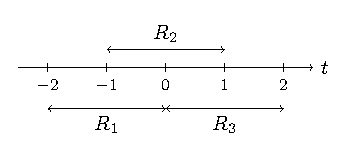
\includegraphics[width=0.8\textwidth]{tikz figures/local RRMC/axis.pdf}
%         \caption{}
%         \label{fig:alternating RRMC}
%     \end{figure}
% \end{example}

% \begin{related}
%     Schwarz alternating method, walk on rectangles paper.
% \end{related}

\section{Brownian Motion}

\begin{definition}[Brownian Motion]
    Define Brownian motion $W_{t}$ as the limit/logical generalization
    when $n \rightarrow \infty$ of following discrete proces defined as:
    \begin{equation}
        \begin{cases}
            X_{t}^{n} = X_{t-\frac{1}{n}}^{n} + Z_{n} \\
            X^{n}_{0}=0
        \end{cases}.
    \end{equation}
    With $Z_{n}\sim N(0,\frac{1}{n})$ i.i.d . From this definition it is easily seen that
    $W_{t} \sim N(0,t)$.
\end{definition}


\begin{lemma}[self-affinity Brownian motion] \label{lem:self affine}
    Brownian motion is self affine as a random proces that means you can cut a small
    part of it move so it starts in $0$ and scale time to the original size
    and space such that the variance stays the same to get back the whole Brownian motion.
\end{lemma}

\begin{equation}
    \forall c \in \mathbb{R}^{+}_{0}: \frac{W_{ct}}{\sqrt{c}} \sim W_{t}.
\end{equation}

\begin{theorem}[Feyman-Kac formula (wikipedia)] \label{thrm:feymankac}

    Consider the partial differential equation
    \begin{equation}
        \frac{\partial u}{\partial t}(x, t)+\mu(x, t) \frac{\partial u}{\partial x}(x, t)+\frac{1}{2} \sigma^2(x, t) \frac{\partial^2 u}{\partial x^2}(x, t)-V(x, t) u(x, t)+f(x, t)=0,
        .
    \end{equation}
    defined for all $x \in \mathbb{R}$ and $t \in[0, T]$, subject to the terminal condition
    \begin{equation}
        u(x, T)=\psi(x),
        .
    \end{equation}
    where $\mu, \sigma, \psi, V, f$ are known functions, $T$ is a parameter, and $u: \mathbb{R} \times[0, T] \rightarrow \mathbb{R}$ is the unknown. Then the Feynman-Kac formula tells us that the solution can be written as a conditional expectation
    \begin{equation}
        u(x, t)=E^Q\left[\int_t^T e^{-\int_t^r V\left(X_\tau, \tau\right) d \tau} f\left(X_r, r\right) d r+e^{-\int_t^T V\left(X_\tau, \tau\right) d \tau} \psi\left(X_T\right) \mid X_t=x\right]
        .
    \end{equation}
    under the probability measure $Q$ such that $X$ is an Itô process driven by the equation
    \begin{equation}
        d X_t=\mu(X, t) d t+\sigma(X, t) d W_t^Q
        .
    \end{equation}
    with $W^Q(t)$ is a Wiener process (also called Brownian motion) under $Q$, and the initial condition for $X(t)$ is $X(t)=x$.
\end{theorem}

\begin{definition}[first passage sampling ] \label{def:first passage}
    In the first passage sampling we try to sample states when a proces
    reaches a boundary or specified state of the system for the first time
    (the first passage). We are specifically interested in
    first passage problem with Brownian motion for a closed time space barrier.
\end{definition}

The first passage distribution of Brownian motion is in fact the boundary
green function for the heat equation this can be easily seen by using the
Feynman-Kac formula (\ref{thrm:feymankac}).

\begin{example}[Euler first passage sampling]
    In this example we naively sample first passage exit point of Brownian motion
    for a parabolic barrier by simulating Brownian motion with the Euler scheme.
    \begin{figure}[ht!]
        \centering
        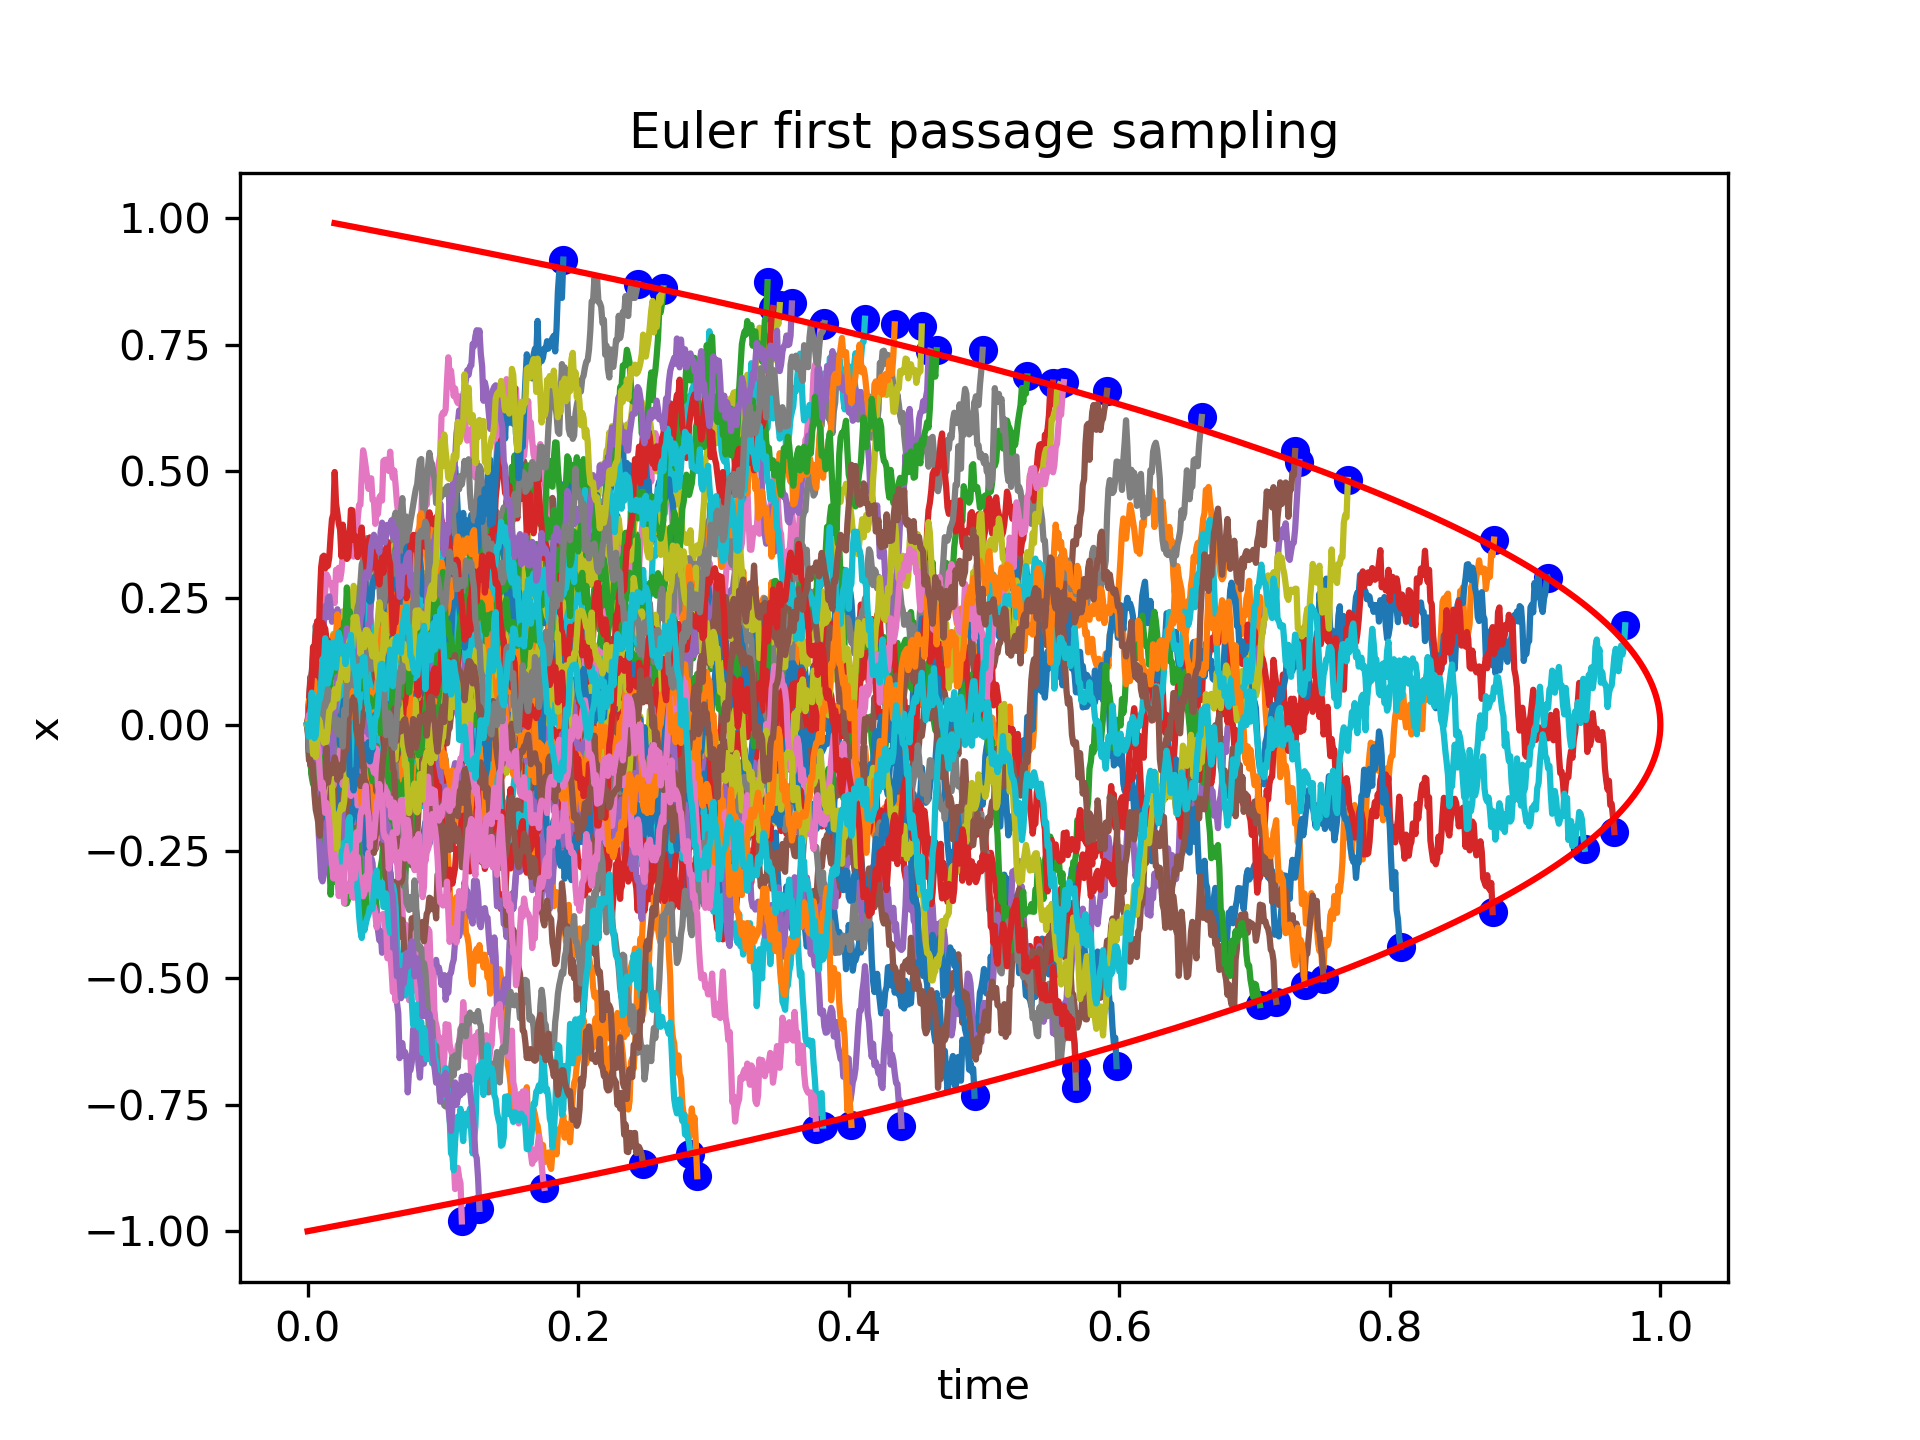
\includegraphics[width=0.8\textwidth]{plots/Euler first passage para.png}
        \caption{ $50$ realizations of Euler first passage sampling with step size $0.001$.}
        \label{fig:Euler first passage para}
    \end{figure}
\end{example}


\begin{technique}[recursive first passage sampling]
    The idea behind recursive first passage sampling is to break down a first passage
    sampling on a bigger domain to contained smaller domains by using the fact you
    can't leave the big domain without leaving the smaller first
    (intermediate value theorem). When you sample the exit from the smaller domain
    it is the start point of a new first passage sampling problem and then you  recurse
    until you are close to the stopping condition.
\end{technique}

\begin{related}[recursive first passage sampling]
    Recursive first passage sampling get discussed in \cite{herrmann_first-passage_2016}
    and extension for processes with jumps in \cite{herrmann_exact_2021}.
\end{related}

\begin{example}[recursive first passage sampling] \label{ex:recursive first passage sampling}
    In this example we recursively first passage sample the exit point of Brownian motion
    for a triangular barrier by resampling and scaling (using (\ref{lem:self affine})) from
    a precomputed Euler scheme to sample a exit point from a parabolic barrier.
    \begin{figure}[ht!]
        \centering
        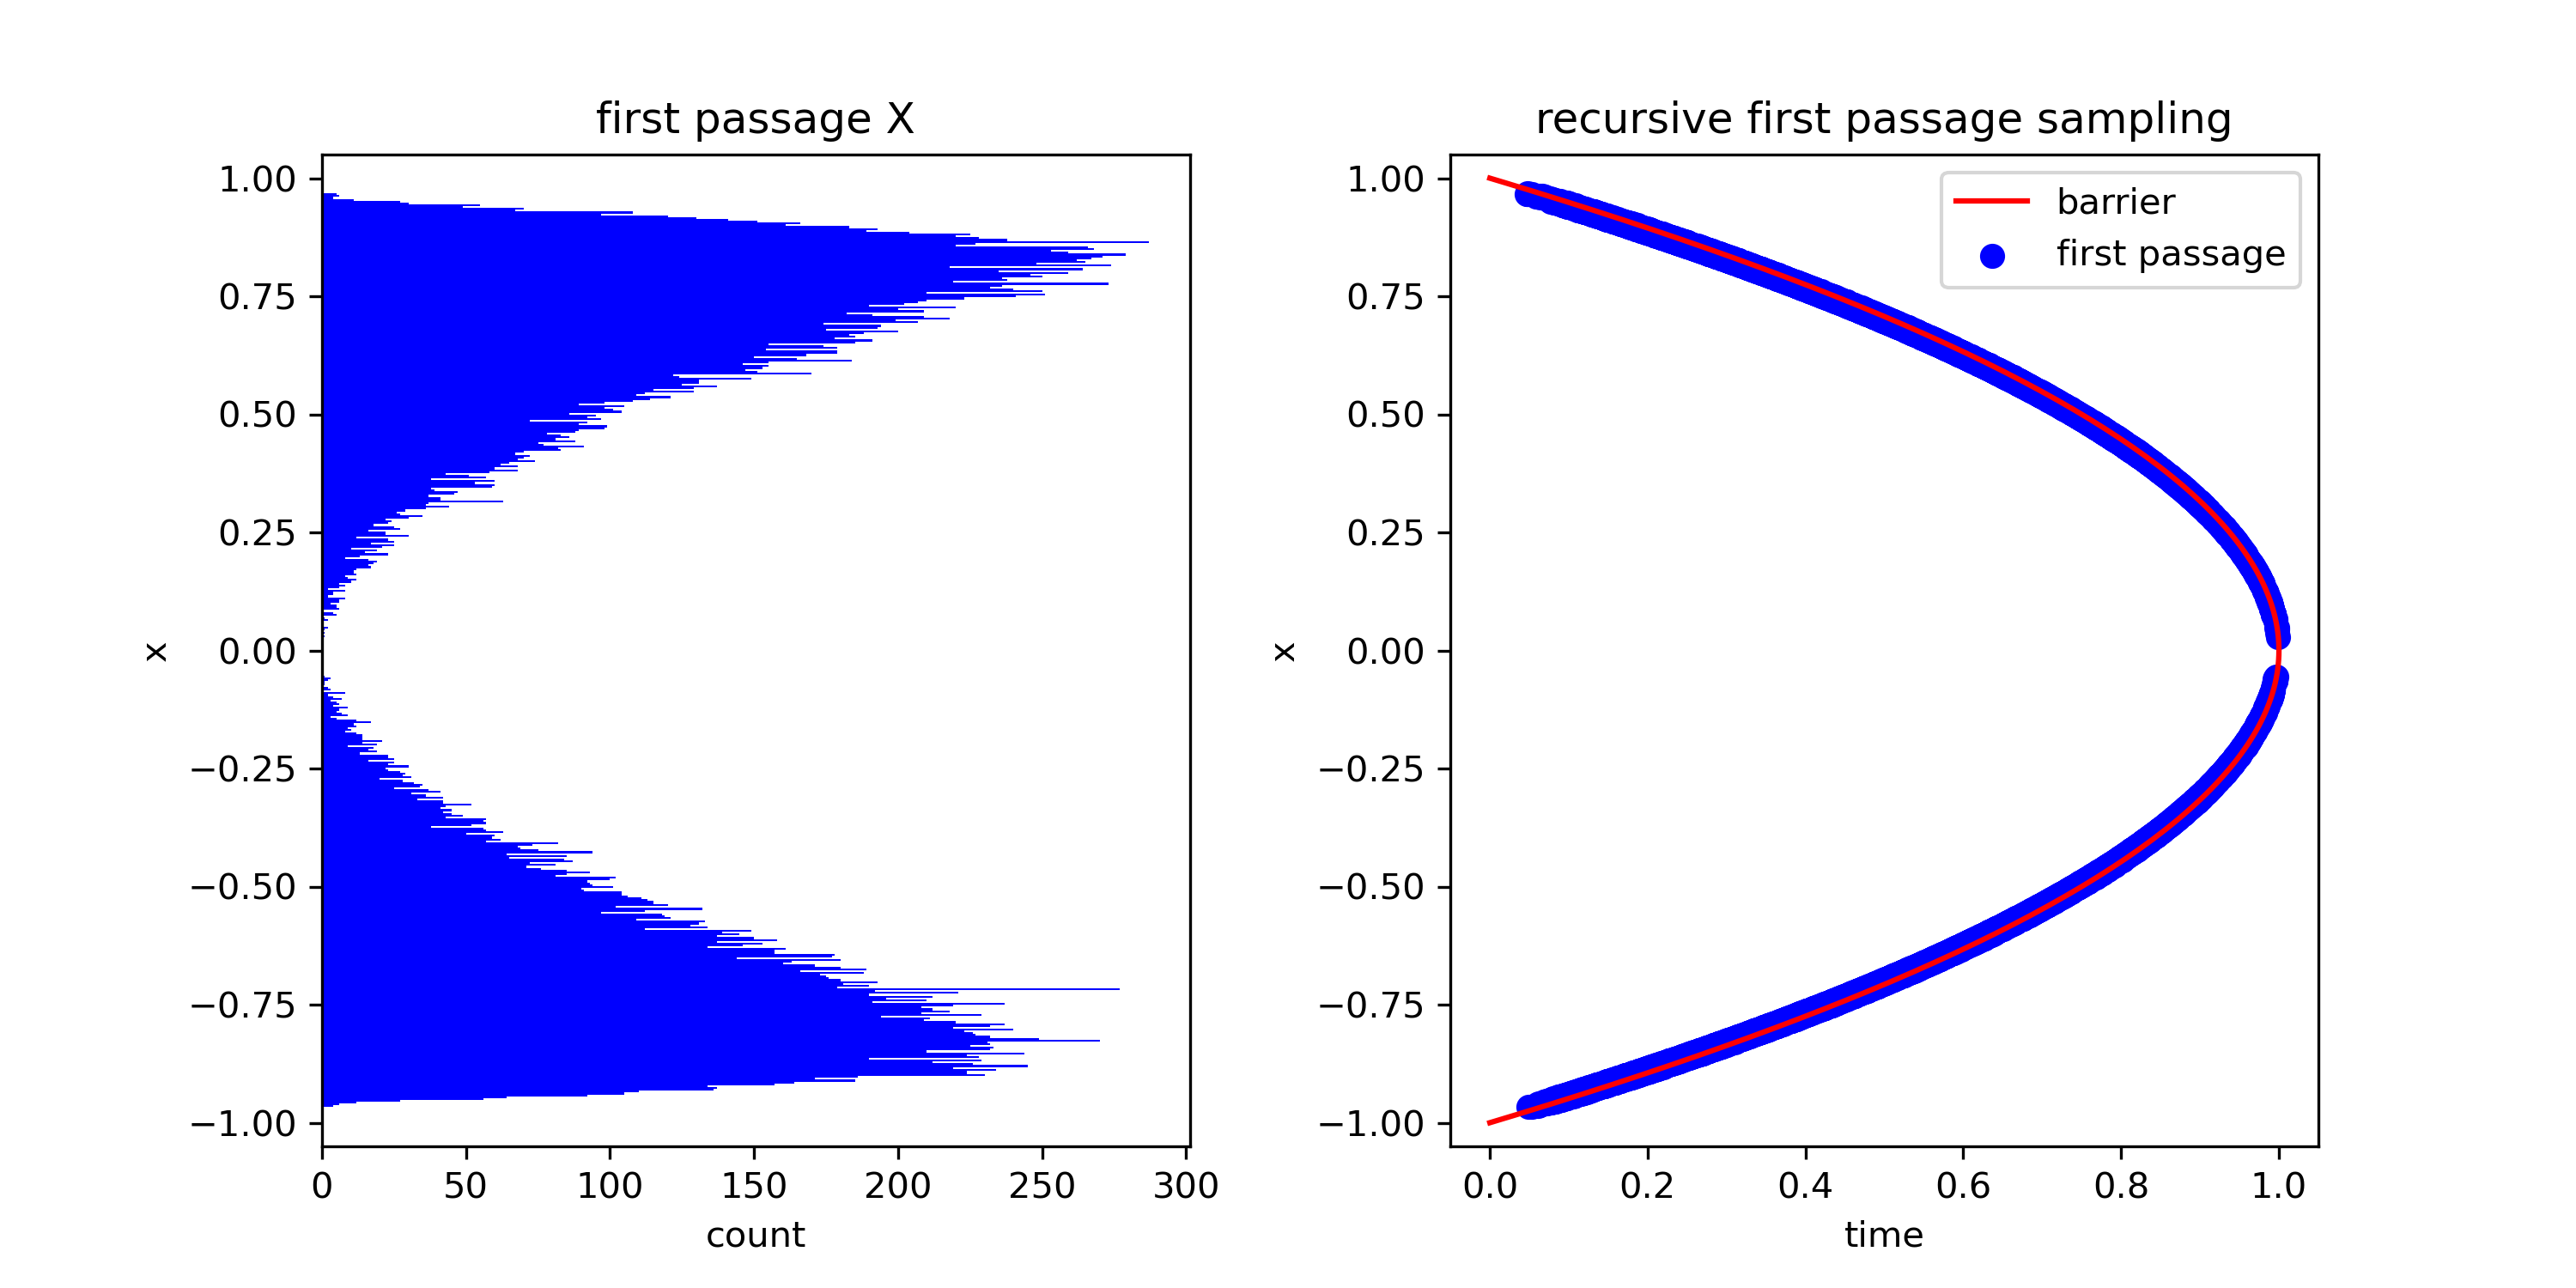
\includegraphics[width=1\textwidth]{plots/recursive first passage para.png}
        \caption{ $50000$ of realizations of recursive first passage sampling.
            The precomputed sample of $1000$ first passages of a triangular barrier
            uses the Euler scheme with step size $0.001$.}
        \label{fig:recursive first passage para}
    \end{figure}
\end{example}

Instead of resampling from a Euler scheme it is also possible
to tabloid the inverse cumulative probability function for the
triangular case. Something similar gets done in \cite{hwang_simulationtabulation_2001}. \\


You can transform first passage sampling problems for others processes back to
Brownian Motion by doing the right time and space bending. For example geometric
Brownian motion can be made into Brownian motion by taking the log. \\


Sometimes we're interested in a specific property of a first passage sampled
path like the max or the average. The naif way would be sampling full paths
and calculating the desired property instead you can sample only the required
information to calculate the desired property. In the case of the max
and the average for example you only need the sample the max/average
of the subpaths and combined that to the max/average of the whole path.\\


\begin{example}[recursive first passage average sampling]
    This is the same as example (\ref{ex:recursive first passage sampling}) but now we have
    to keep track of the average.

    \begin{figure}[ht!]
        \centering
        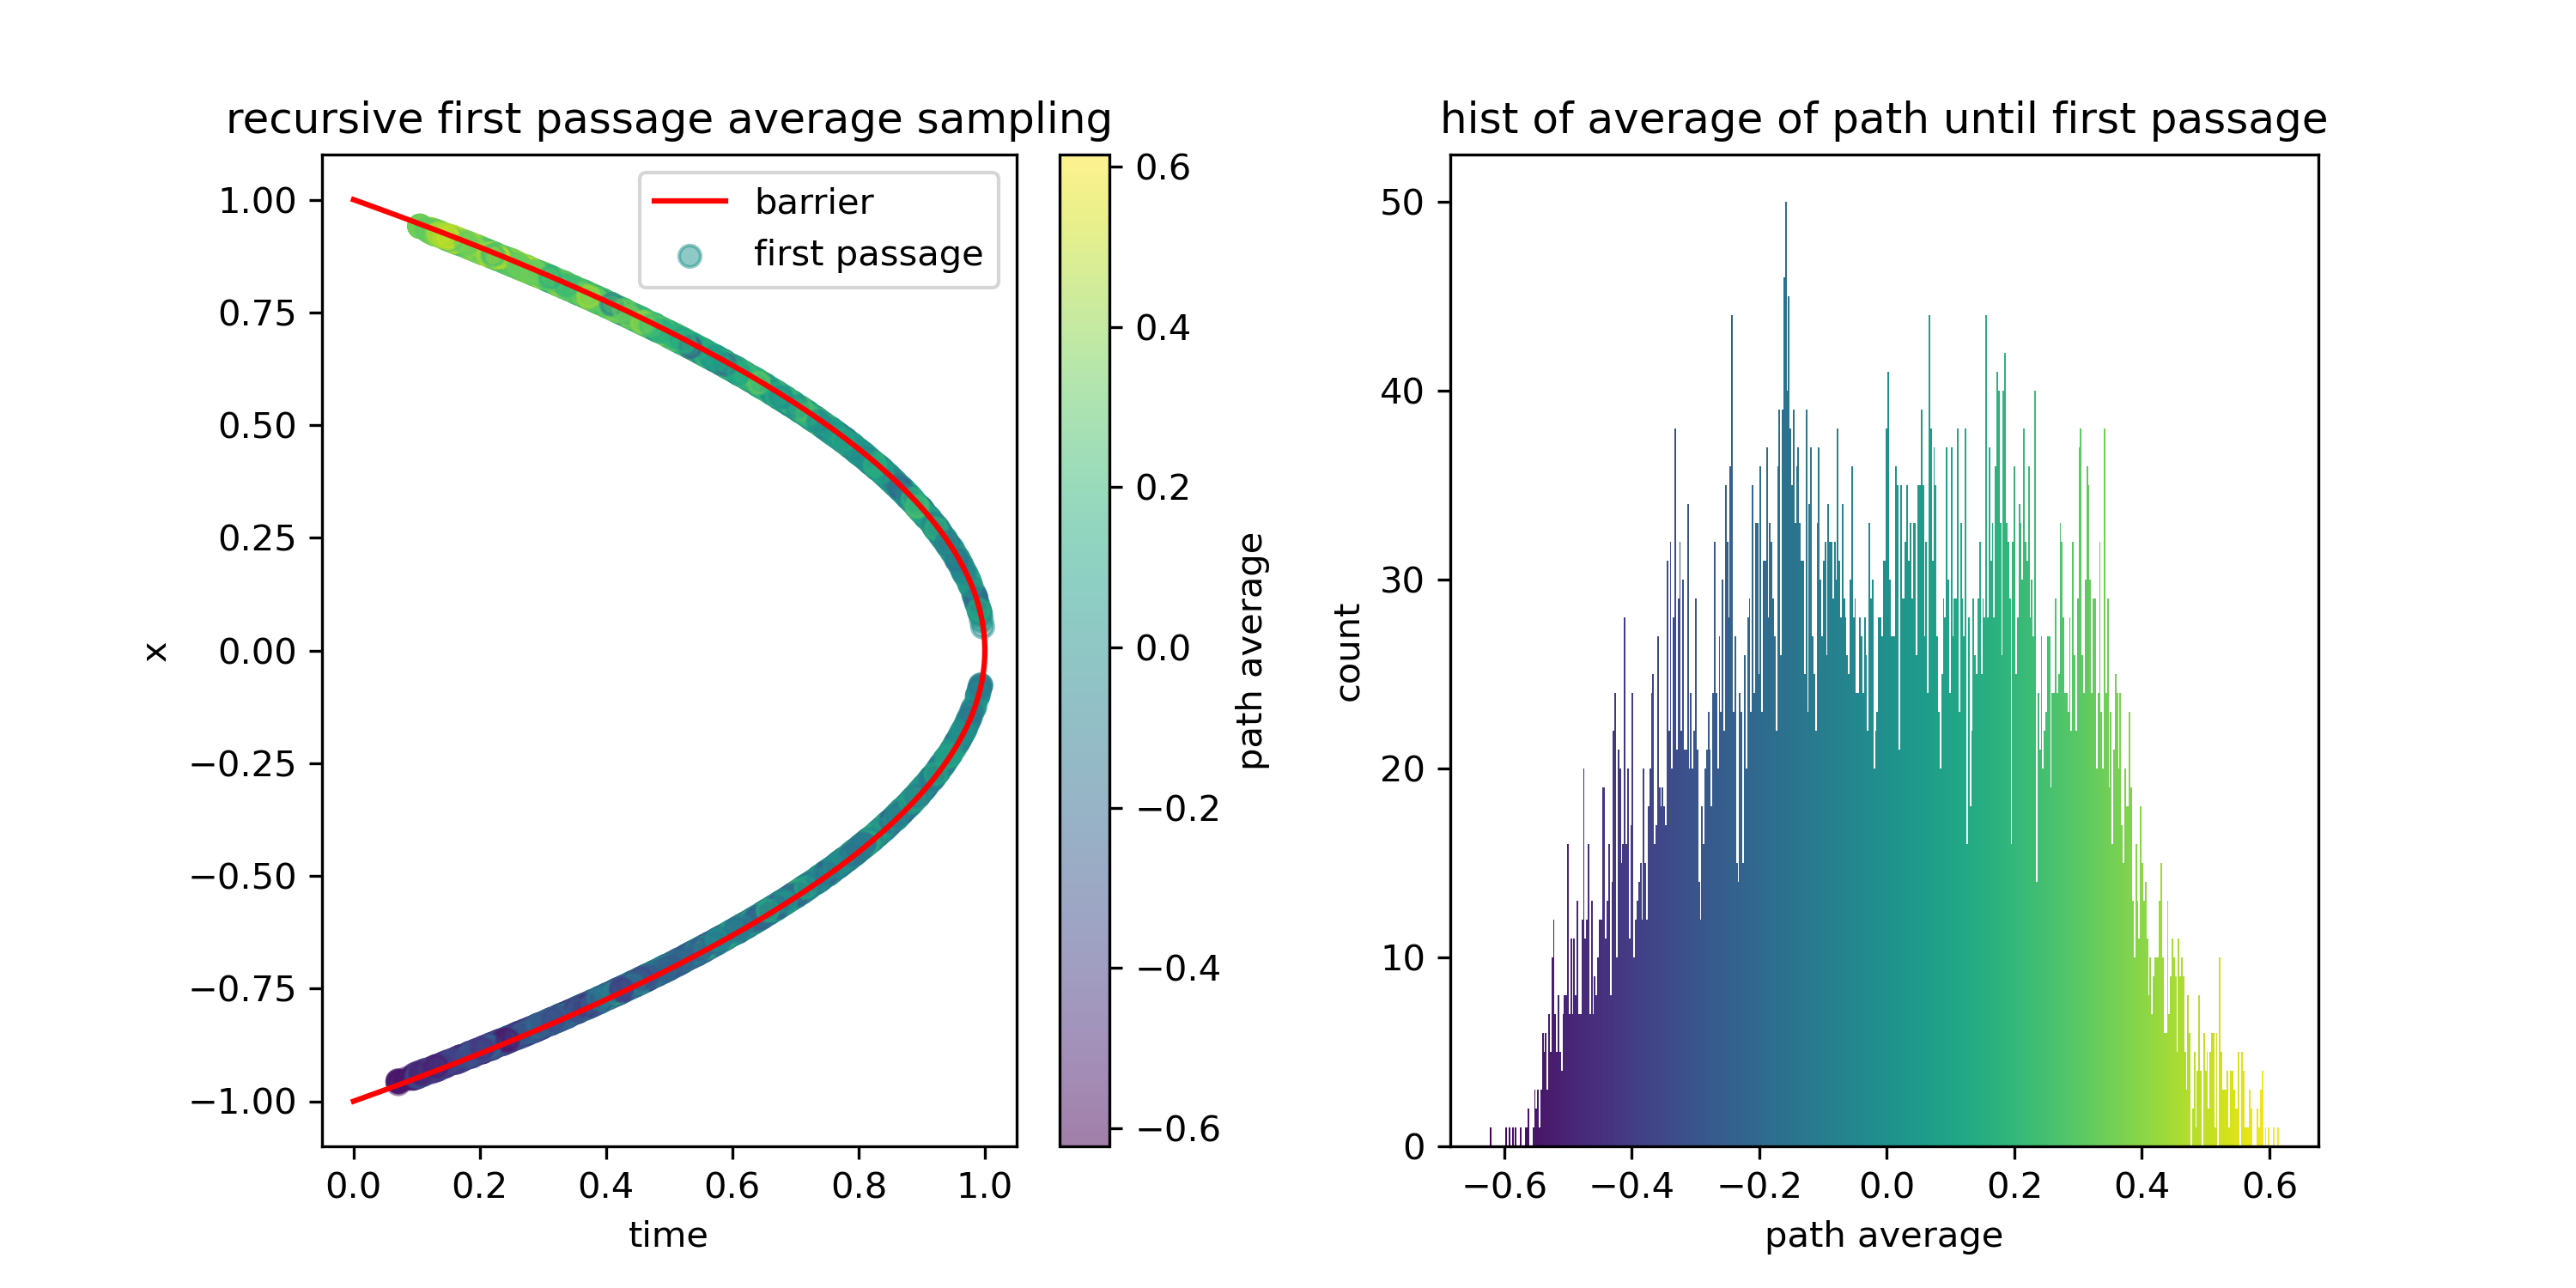
\includegraphics[width=1\textwidth]{plots/recursive first passage average para.png}
        \caption{ $10000$ of realizations of recursive first passage sampling (for the average).
            The precomputed sample of $1000$ first passages and averages of a triangular barrier
            uses the Euler scheme with step size $0.001$.}
        \label{fig:recursive first passage average para}
    \end{figure}
\end{example}

Doing the same thing for geometric Brownian motion is difficult because the average
behaves bad under transformation unlike the max. You can think of the average
as an extra dimension to keep track of. What you would need  for geometric
Brownian motion is the  first passage distribution of the average and exit
point for every different position of the begin point for subpaths.\\
And nothing holds you back of changing methods midway if you didn't
the precompute a situation.

\begin{technique}[path stitching]
    Instead of thinking in sampling first passage points you can also sample
    whole paths to the first passage. The same way as before you need to be
    able to generate paths for a simple first passage problem and "stich"
    these paths together into one for a complicated one.
\end{technique}

\begin{example}[path stitching parabola]
    This is the same as example (\ref{ex:recursive first passage sampling}) but now we have
    to keep track of the whole resampled Euler scheme generated paths.

    \begin{figure}[ht!]
        \centering
        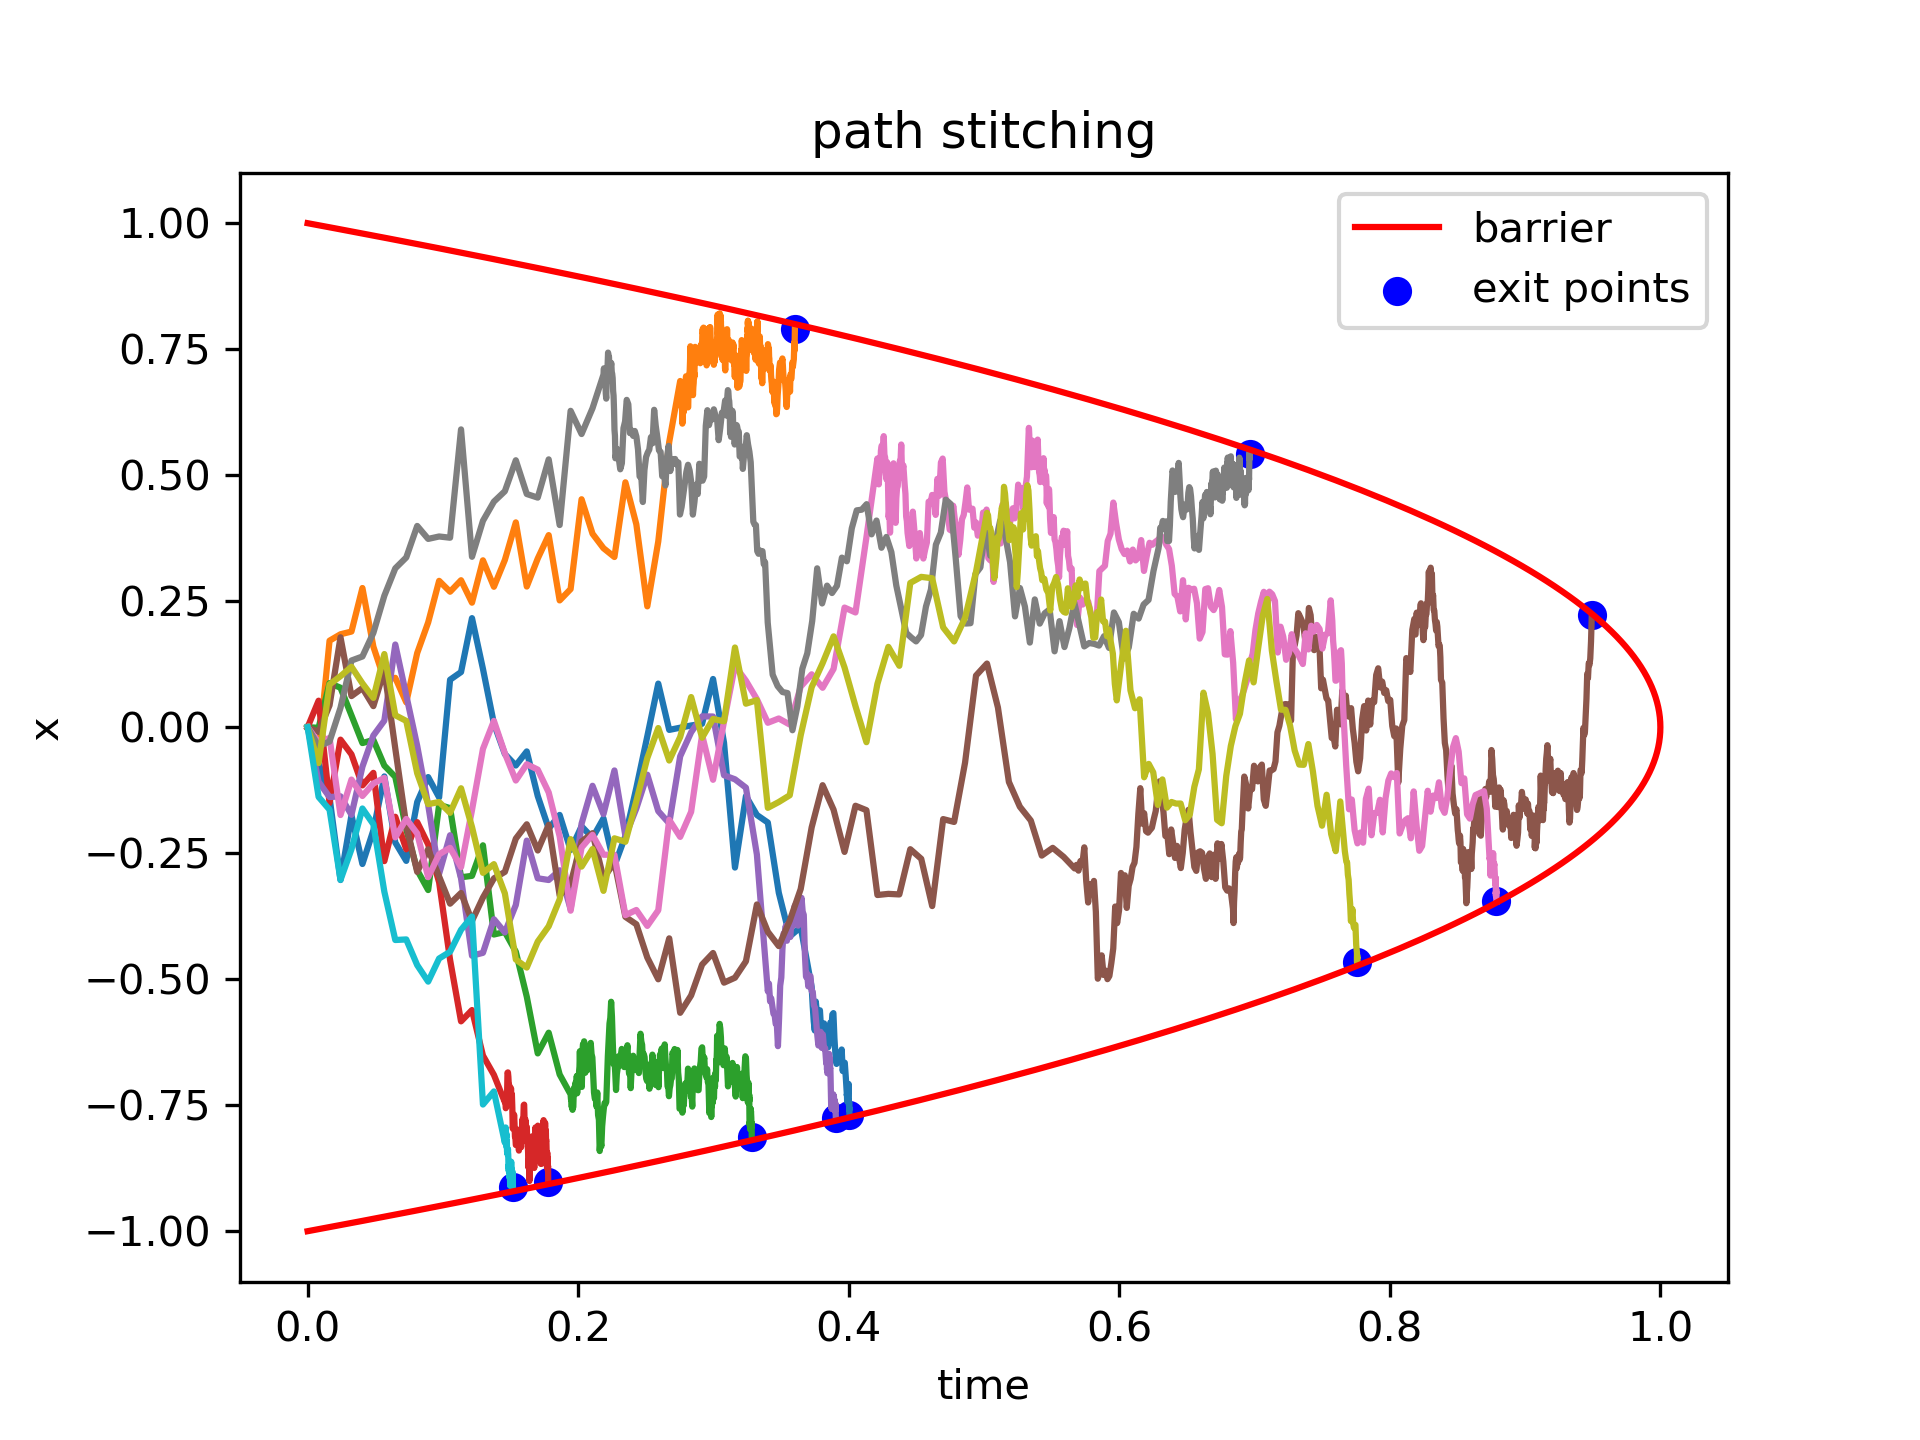
\includegraphics[width=0.8\textwidth]{plots/path stitching para.png}
        \caption{ $10$ paths build with path stitching build out of
            precomputed Euler scheme generated paths with stepsize $0.01$.}
        \label{fig:path stitching para}
    \end{figure}
\end{example}

For plotting the path we needed to accesses to all of its points.  An advantage
over normally generating paths is that a path can be represented by its subpaths
and their scalings requiring way less memory then a full path. This can be useful
in case where the whole path isn't needed. Even if  accesses to the whole
path is needed this can be done in a slightly more efficient manor
then a normal Euler scheme because it can almost be done in parallel
vs step for step generation. The only downsides are that the time
steps are inhomogeneous and it requires a precomputation. \\

A way around scaling base samples is limiting scaling to a
discrete set and pick the biggest scaling that fits, instead
of generating base samples for $1$ scale and scaling it dynamically
precompute all the discrete scalings. \\

Similar precomputing tricks can be used for geometric Brownian motion
requiring and extra dimension of precomputing based on transformations.

\begin{related}[path stitching]
    Path stitching appears frequently in rendering and also in \cite{das_sarma_fast_2015}
    and \cite{ji_reusing_2012}.
\end{related}

\newpage
\printbibliography
\newpage

% \section{Appendix}
% Derivation of the green functions and some expressions.
\end{document}
